% Slides for Software Carpentry workshop at Tulane
% January 2015 - New Orleans, LA
%
% Original slides by: Karthik Ram, karthik.ram@gmail.com
% Modified by: Naupaka Zimmerman, naupaka@gmail.com
% Licence, CC-BY 4.0

\documentclass{beamer}\usepackage[]{graphicx}\usepackage[]{color}
%% maxwidth is the original width if it is less than linewidth
%% otherwise use linewidth (to make sure the graphics do not exceed the margin)
\makeatletter
\def\maxwidth{ %
  \ifdim\Gin@nat@width>\linewidth
    \linewidth
  \else
    \Gin@nat@width
  \fi
}
\makeatother

\definecolor{fgcolor}{rgb}{0.345, 0.345, 0.345}
\newcommand{\hlnum}[1]{\textcolor[rgb]{0.686,0.059,0.569}{#1}}%
\newcommand{\hlstr}[1]{\textcolor[rgb]{0.192,0.494,0.8}{#1}}%
\newcommand{\hlcom}[1]{\textcolor[rgb]{0.678,0.584,0.686}{\textit{#1}}}%
\newcommand{\hlopt}[1]{\textcolor[rgb]{0,0,0}{#1}}%
\newcommand{\hlstd}[1]{\textcolor[rgb]{0.345,0.345,0.345}{#1}}%
\newcommand{\hlkwa}[1]{\textcolor[rgb]{0.161,0.373,0.58}{\textbf{#1}}}%
\newcommand{\hlkwb}[1]{\textcolor[rgb]{0.69,0.353,0.396}{#1}}%
\newcommand{\hlkwc}[1]{\textcolor[rgb]{0.333,0.667,0.333}{#1}}%
\newcommand{\hlkwd}[1]{\textcolor[rgb]{0.737,0.353,0.396}{\textbf{#1}}}%

\usepackage{framed}
\makeatletter
\newenvironment{kframe}{%
 \def\at@end@of@kframe{}%
 \ifinner\ifhmode%
  \def\at@end@of@kframe{\end{minipage}}%
  \begin{minipage}{\columnwidth}%
 \fi\fi%
 \def\FrameCommand##1{\hskip\@totalleftmargin \hskip-\fboxsep
 \colorbox{shadecolor}{##1}\hskip-\fboxsep
     % There is no \\@totalrightmargin, so:
     \hskip-\linewidth \hskip-\@totalleftmargin \hskip\columnwidth}%
 \MakeFramed {\advance\hsize-\width
   \@totalleftmargin\z@ \linewidth\hsize
   \@setminipage}}%
 {\par\unskip\endMakeFramed%
 \at@end@of@kframe}
\makeatother

\definecolor{shadecolor}{rgb}{.97, .97, .97}
\definecolor{messagecolor}{rgb}{0, 0, 0}
\definecolor{warningcolor}{rgb}{1, 0, 1}
\definecolor{errorcolor}{rgb}{1, 0, 0}
\newenvironment{knitrout}{}{} % an empty environment to be redefined in TeX

\usepackage{alltt}
\usepackage{listings}
\usepackage{inconsolata}
\setbeamertemplate{frametitle}[default][center]
\usepackage{url}
\usepackage{color}
\setcounter{secnumdepth}{-1}
\usetheme{default}
\defbeamertemplate*{title page}{customized}[1][]
{
  \begin{center}
  \usebeamerfont{title}\inserttitle\par
  \usebeamerfont{subtitle}\usebeamercolor[fg]{subtitle}\insertsubtitle\par
  \bigskip
  \bigskip
  \bigskip
  \usebeamerfont{author}\insertauthor\par
  \usebeamerfont{date}\insertdate\par
  \end{center}
}
\addtobeamertemplate{frametitle}{\vspace*{0.5cm}}{}

% --------------------------------------------------------------
% --------------------------------------------------------------
% --------------------------------------------------------------

% Setting up some knitr options


% --------------------------------------------------------------
% --------------------------------------------------------------
% --------------------------------------------------------------
\IfFileExists{upquote.sty}{\usepackage{upquote}}{}
\begin{document}
% \SweaveOpts{concordance=TRUE} % deprecated

\title{Data Visualization Using R \& ggplot2}
\author{Naupaka Zimmerman (@naupakaz) \linebreak Andrew Tredennick (@ATredennick) \linebreak \linebreak Hat tip to Karthik Ram (@\_inundata) for original slides \linebreak}
\date{January 27, 2015}
\maketitle

% --------------------------------------------------------------

\begin{frame}[fragile]
\frametitle{Some housekeeping}
Install some packages
\begin{knitrout}\footnotesize
\definecolor{shadecolor}{rgb}{0.969, 0.969, 0.969}\color{fgcolor}\begin{kframe}
\begin{alltt}
\hlkwd{install.packages}\hlstd{(}\hlstr{"ggplot2"}\hlstd{,} \hlkwc{dependencies} \hlstd{=} \hlnum{TRUE}\hlstd{)}
\hlkwd{install.packages}\hlstd{(}\hlstr{"plyr"}\hlstd{)}
\hlkwd{install.packages}\hlstd{(}\hlstr{"ggthemes"}\hlstd{)}
\hlkwd{install.packages}\hlstd{(}\hlstr{"reshape2"}\hlstd{)}
\end{alltt}
\end{kframe}
\end{knitrout}
\end{frame}

% --------------------------------------------------------------
% --------------------------------------------------------------

\section*{Why \texttt{ggplot2}?}
\frame{\sectionpage}

% --------------------------------------------------------------
% --------------------------------------------------------------

\begin{frame}[fragile]
\frametitle{Why \texttt{ggplot2}?}
\begin{itemize}
\item More elegant \& compact code than with base graphics\\
\item More aesthetically pleasing defaults than lattice\\
\item Very powerful for exploratory data analysis\\
\end{itemize}
\end{frame}

% --------------------------------------------------------------

\begin{frame}[fragile]
\frametitle{Why \texttt{ggplot2}?}
\begin{itemize}
\item `gg' is for `grammar of graphics' (term by Lee Wilkinson)\\
\item A set of terms that defines the basic components of a plot\\
\item Used to produce figures using coherant, consistant syntax\\
\end{itemize}
\end{frame}

% --------------------------------------------------------------

\begin{frame}[fragile]
\frametitle{Why \texttt{ggplot2}?}
\begin{itemize}
\item Supports a continuum of expertise:
\item Easy to get started, plenty of power for complex figures 
\end{itemize}
\end{frame}

% --------------------------------------------------------------
% --------------------------------------------------------------

\section*{The Grammar}
\frame{\sectionpage}

% --------------------------------------------------------------
% --------------------------------------------------------------

\begin{frame}[fragile]
\frametitle{Some terminology}
\begin{columns}[t]

\begin{column}[T]{3cm}
\begin{itemize}
    \item \textbf{data}
\end{itemize}
\end{column}

\begin{column}[T]{8cm}
\begin{itemize}
    \item Must be a data.frame
    \item Gets pulled into the ggplot() object
\end{itemize}
\end{column}

\end{columns}
\end{frame}

% --------------------------------------------------------------

\begin{frame}[fragile]
\frametitle{The iris dataset}
\begin{knitrout}\footnotesize
\definecolor{shadecolor}{rgb}{0.969, 0.969, 0.969}\color{fgcolor}\begin{kframe}
\begin{alltt}
\hlkwd{head}\hlstd{(iris)}
\end{alltt}
\begin{verbatim}
##   Sepal.Length Sepal.Width Petal.Length Petal.Width Species
## 1          5.1         3.5          1.4         0.2  setosa
## 2          4.9         3.0          1.4         0.2  setosa
## 3          4.7         3.2          1.3         0.2  setosa
## 4          4.6         3.1          1.5         0.2  setosa
## 5          5.0         3.6          1.4         0.2  setosa
## 6          5.4         3.9          1.7         0.4  setosa
\end{verbatim}
\end{kframe}
\end{knitrout}
\end{frame}

% --------------------------------------------------------------

\begin{frame}[fragile]
\frametitle{\texttt{plyr} and \texttt{reshape} are key for using \texttt{R}}
These two packages are the swiss army knives of \texttt{R}.
\begin{itemize}
\item \texttt{plyr}
    \begin{enumerate}
    \item ddply (data frame to data frame ply)
        \begin{enumerate}
        \item split
        \item apply
        \item combine
        \end{enumerate}
    \item llply (list to list ply)
    \item join
    \end{enumerate}
\end{itemize}
\end{frame}

% --------------------------------------------------------------

\begin{frame}[fragile]
\frametitle{\texttt{plyr}}
\begin{knitrout}\footnotesize
\definecolor{shadecolor}{rgb}{0.969, 0.969, 0.969}\color{fgcolor}\begin{kframe}
\begin{alltt}
\hlstd{iris[}\hlnum{1}\hlopt{:}\hlnum{2}\hlstd{, ]}
\end{alltt}
\begin{verbatim}
##   Sepal.Length Sepal.Width Petal.Length Petal.Width Species
## 1          5.1         3.5          1.4         0.2  setosa
## 2          4.9         3.0          1.4         0.2  setosa
\end{verbatim}
\begin{alltt}
\hlcom{# Note the use of the '.' function to allow 'Species' to be used }
\hlcom{# without quoting}
\hlkwd{ddply}\hlstd{(iris,} \hlkwd{.}\hlstd{(Species), summarize,}
      \hlkwc{mean.Sep.Wid} \hlstd{=} \hlkwd{mean}\hlstd{(Sepal.Width,} \hlkwc{na.rm} \hlstd{=} \hlnum{TRUE}\hlstd{))}
\end{alltt}
\begin{verbatim}
##      Species mean.Sep.Wid
## 1     setosa        3.428
## 2 versicolor        2.770
## 3  virginica        2.974
\end{verbatim}
\end{kframe}
\end{knitrout}
\end{frame}

% --------------------------------------------------------------


\begin{frame}[fragile]
\frametitle{\texttt{plyr} and \texttt{reshape} are key for using \texttt{R}}
These two packages are the swiss army knives of \texttt{R}.
\begin{itemize}
    \item \texttt{reshape}
    \begin{enumerate}
    \item melt
    \item dcast (data frame output)
    \item acast (vector/matrix/array output)
    \end{enumerate}
\end{itemize}
\end{frame}

% --------------------------------------------------------------

\begin{frame}[fragile]
\frametitle{\texttt{reshape2}}
\begin{knitrout}\footnotesize
\definecolor{shadecolor}{rgb}{0.969, 0.969, 0.969}\color{fgcolor}\begin{kframe}
\begin{alltt}
\hlstd{iris[}\hlnum{1}\hlopt{:}\hlnum{2}\hlstd{, ]}
\end{alltt}
\begin{verbatim}
##   Sepal.Length Sepal.Width Petal.Length Petal.Width Species
## 1          5.1         3.5          1.4         0.2  setosa
## 2          4.9         3.0          1.4         0.2  setosa
\end{verbatim}
\begin{alltt}
\hlstd{df}  \hlkwb{<-} \hlkwd{melt}\hlstd{(iris,} \hlkwc{id.vars} \hlstd{=} \hlstr{"Species"}\hlstd{)}
\hlstd{df[}\hlnum{1}\hlopt{:}\hlnum{2}\hlstd{, ]}
\end{alltt}
\begin{verbatim}
##   Species     variable value
## 1  setosa Sepal.Length   5.1
## 2  setosa Sepal.Length   4.9
\end{verbatim}
\end{kframe}
\end{knitrout}
\end{frame}

% --------------------------------------------------------------

\begin{frame}[fragile]
\frametitle{\texttt{reshape2}}
\begin{knitrout}\footnotesize
\definecolor{shadecolor}{rgb}{0.969, 0.969, 0.969}\color{fgcolor}\begin{kframe}
\begin{alltt}
\hlstd{df[}\hlnum{1}\hlopt{:}\hlnum{2}\hlstd{, ]}
\end{alltt}
\begin{verbatim}
##   Species     variable value
## 1  setosa Sepal.Length   5.1
## 2  setosa Sepal.Length   4.9
\end{verbatim}
\begin{alltt}
\hlkwd{dcast}\hlstd{(df, Species} \hlopt{~} \hlstd{variable, mean)}
\end{alltt}
\begin{verbatim}
##      Species Sepal.Length Sepal.Width Petal.Length
## 1     setosa        5.006       3.428        1.462
## 2 versicolor        5.936       2.770        4.260
## 3  virginica        6.588       2.974        5.552
##   Petal.Width
## 1       0.246
## 2       1.326
## 3       2.026
\end{verbatim}
\end{kframe}
\end{knitrout}
\end{frame}

% --------------------------------------------------------------
% --------------------------------------------------------------

\section*{Aesthetics}
\frame{\sectionpage}

% --------------------------------------------------------------
% --------------------------------------------------------------


\begin{frame}[fragile]
\frametitle{Some terminology}
\begin{columns}[t]

\begin{column}[T]{3cm}
\begin{itemize}
    \item \textbf{\color{gray}data}
    \item \textbf{aes}thetics
\end{itemize}
\end{column}

\begin{column}[T]{8cm}
\begin{itemize}
    \item \textbf{How your data are represented visually}
        \begin{itemize}
        \item \emph{a.k.a. mapping}
        \end{itemize}
    \item which data on the x
    \item which data on the y
    \item but also: {\color{red}color}, {\LARGE{size}}, shape, transparency
\end{itemize}
\end{column}

\end{columns}
\end{frame}

% --------------------------------------------------------------

\begin{frame}[fragile]
\frametitle{Let's try an example}
\begin{knitrout}\footnotesize
\definecolor{shadecolor}{rgb}{0.969, 0.969, 0.969}\color{fgcolor}\begin{kframe}
\begin{alltt}
\hlstd{myplot} \hlkwb{<-} \hlkwd{ggplot}\hlstd{(}\hlkwc{data} \hlstd{= iris,} \hlkwd{aes}\hlstd{(}\hlkwc{x} \hlstd{= Sepal.Length,} \hlkwc{y} \hlstd{= Sepal.Width))}
\hlkwd{summary}\hlstd{(myplot)}
\end{alltt}
\begin{verbatim}
## data: Sepal.Length, Sepal.Width, Petal.Length,
##   Petal.Width, Species [150x5]
## mapping:  x = Sepal.Length, y = Sepal.Width
## faceting: facet_null()
\end{verbatim}
\end{kframe}
\end{knitrout}
\end{frame}

% --------------------------------------------------------------
% --------------------------------------------------------------

\section*{Geoms}
\frame{\sectionpage}

% --------------------------------------------------------------
% --------------------------------------------------------------

\begin{frame}[fragile]
\frametitle{Some terminology}
\begin{columns}[t]

\begin{column}[T]{3cm}
\begin{itemize}
    \item \textbf{\color{gray}data}
    \item \textbf{\color{gray}aesthetics}
    \item \textbf{geom}etry
\end{itemize}
\end{column}

\begin{column}[T]{8cm}
\begin{itemize}
    \item \textbf{The geometric objects in the plot}
    \item points, lines, polygons, etc
    \item shortcut functions: geom\_point(), geom\_bar(), geom\_line()
\end{itemize}
\end{column}

\end{columns}
\end{frame}

% --------------------------------------------------------------

\begin{frame}[fragile]
\frametitle{Basic structure}
\begin{knitrout}\footnotesize
\definecolor{shadecolor}{rgb}{0.969, 0.969, 0.969}\color{fgcolor}\begin{kframe}
\begin{alltt}
\hlkwd{ggplot}\hlstd{(}\hlkwc{data} \hlstd{= iris,} \hlkwd{aes}\hlstd{(}\hlkwc{x} \hlstd{= Sepal.Length,} \hlkwc{y} \hlstd{= Sepal.Width))}
    \hlopt{+} \hlkwd{geom_point}\hlstd{()}

\hlstd{myplot} \hlkwb{<-} \hlkwd{ggplot}\hlstd{(}\hlkwc{data} \hlstd{= iris,} \hlkwd{aes}\hlstd{(}\hlkwc{x} \hlstd{= Sepal.Length,} \hlkwc{y} \hlstd{= Sepal.Width))}
\hlstd{myplot} \hlopt{+} \hlkwd{geom_point}\hlstd{()}
\end{alltt}
\end{kframe}
\end{knitrout}
\begin{itemize}
\item Specify the data and variables inside the \texttt{ggplot} function.
\item Anything else that goes in here becomes a global setting.
\item Then add layers: geometric objects, statistical models, and facets.
\end{itemize}
\end{frame}

% --------------------------------------------------------------

\begin{frame}[fragile]
\frametitle{Quick note}
\begin{itemize}
\item Never use \texttt{qplot} - short for quick plot.
\item You`ll end up unlearning and relearning a good bit.
\end{itemize}

\end{frame}

% --------------------------------------------------------------

\begin{frame}[fragile]
\frametitle{Let's try an example}
\begin{knitrout}\footnotesize
\definecolor{shadecolor}{rgb}{0.969, 0.969, 0.969}\color{fgcolor}\begin{kframe}
\begin{alltt}
\hlkwd{ggplot}\hlstd{(}\hlkwc{data} \hlstd{= iris,} \hlkwd{aes}\hlstd{(}\hlkwc{x} \hlstd{= Sepal.Length,} \hlkwc{y} \hlstd{= Sepal.Width))} \hlopt{+}
    \hlkwd{geom_point}\hlstd{()}
\end{alltt}
\end{kframe}

{\centering 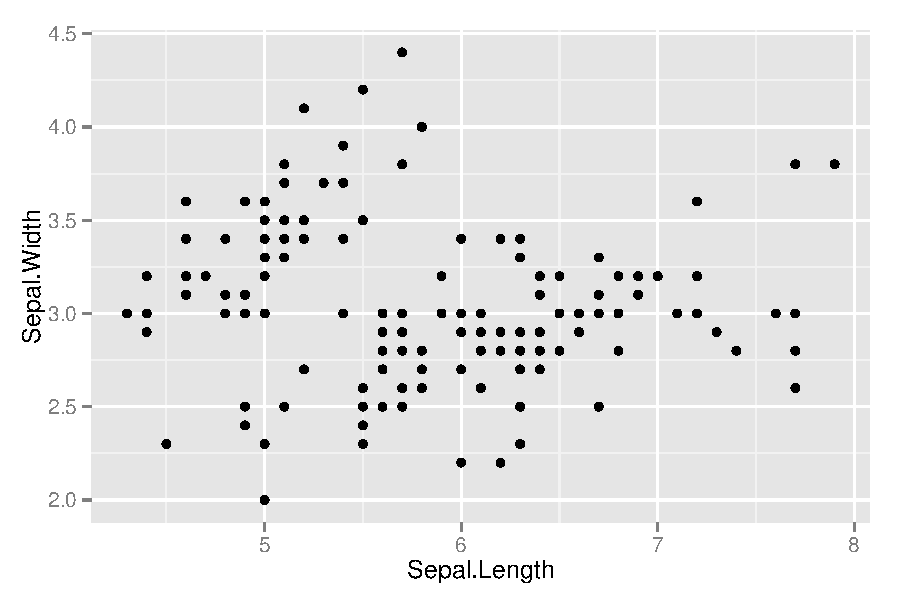
\includegraphics[width=.75\linewidth]{figure/first_plot_-1} 

}



\end{knitrout}
\end{frame}

% --------------------------------------------------------------

\begin{frame}[fragile]
\frametitle{Changing the aesthetics of a geom: \\Increase the size of points}
\begin{knitrout}\footnotesize
\definecolor{shadecolor}{rgb}{0.969, 0.969, 0.969}\color{fgcolor}\begin{kframe}
\begin{alltt}
\hlkwd{ggplot}\hlstd{(}\hlkwc{data} \hlstd{= iris,} \hlkwd{aes}\hlstd{(}\hlkwc{x} \hlstd{= Sepal.Length,} \hlkwc{y} \hlstd{= Sepal.Width))} \hlopt{+}
    \hlkwd{geom_point}\hlstd{(}\hlkwc{size} \hlstd{=} \hlnum{3}\hlstd{)}
\end{alltt}
\end{kframe}

{\centering 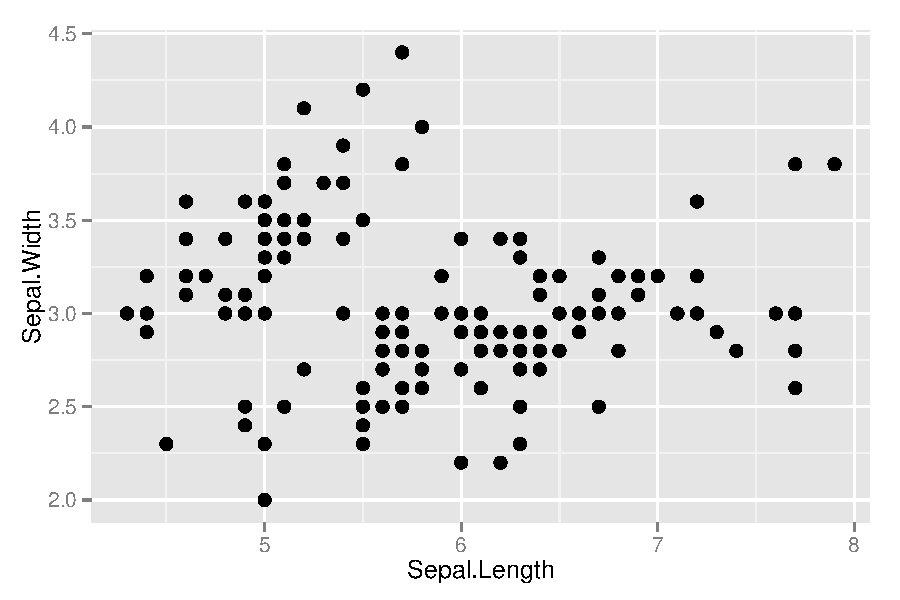
\includegraphics[width=.75\linewidth]{figure/first_plot_size_-1} 

}



\end{knitrout}
\end{frame}

% --------------------------------------------------------------

\begin{frame}[fragile]
\frametitle{Changing the aesthetics of a geom: \\Add some color}
\begin{knitrout}\footnotesize
\definecolor{shadecolor}{rgb}{0.969, 0.969, 0.969}\color{fgcolor}\begin{kframe}
\begin{alltt}
\hlkwd{ggplot}\hlstd{(iris,} \hlkwd{aes}\hlstd{(Sepal.Length, Sepal.Width,} \hlkwc{color} \hlstd{= Species))} \hlopt{+}
    \hlkwd{geom_point}\hlstd{(}\hlkwc{size} \hlstd{=} \hlnum{3}\hlstd{)}
\end{alltt}
\end{kframe}

{\centering 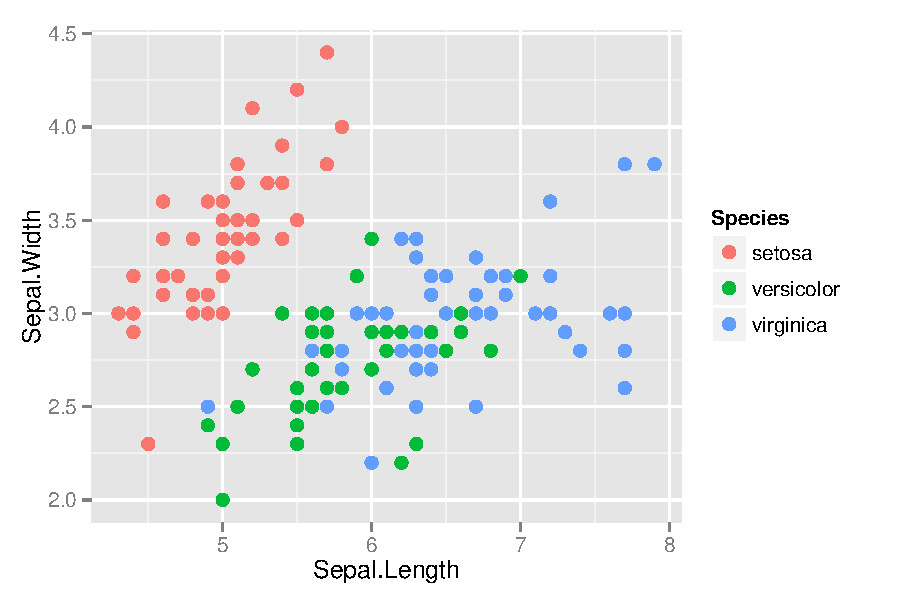
\includegraphics[width=.75\linewidth]{figure/first_plot_color_-1} 

}



\end{knitrout}
\end{frame}

% --------------------------------------------------------------

\begin{frame}[fragile]
\frametitle{Changing the aesthetics of a geom: \\Differentiate points by shape}
\begin{knitrout}\footnotesize
\definecolor{shadecolor}{rgb}{0.969, 0.969, 0.969}\color{fgcolor}\begin{kframe}
\begin{alltt}
\hlkwd{ggplot}\hlstd{(iris,} \hlkwd{aes}\hlstd{(Sepal.Length, Sepal.Width,} \hlkwc{color} \hlstd{= Species))} \hlopt{+}
    \hlkwd{geom_point}\hlstd{(}\hlkwd{aes}\hlstd{(}\hlkwc{shape} \hlstd{= Species),} \hlkwc{size} \hlstd{=} \hlnum{3}\hlstd{)}
\hlcom{# Why aes(shape = Species)?}
\end{alltt}
\end{kframe}

{\centering 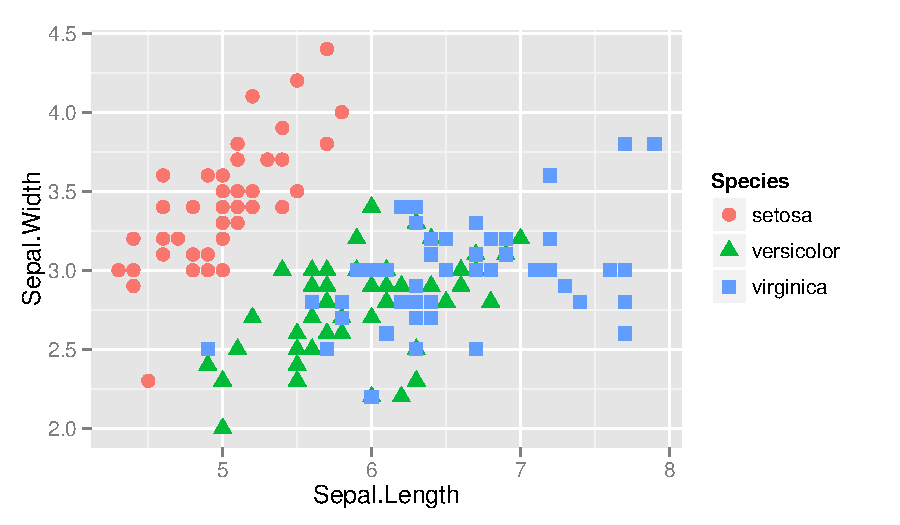
\includegraphics[width=.75\linewidth]{figure/first_plot_shape_-1} 

}



\end{knitrout}
\end{frame}

% --------------------------------------------------------------

\begin{frame}[fragile]
\frametitle{Exercise 1}
\begin{knitrout}\footnotesize
\definecolor{shadecolor}{rgb}{0.969, 0.969, 0.969}\color{fgcolor}\begin{kframe}
\begin{alltt}
\hlcom{# Make a small sample of the diamonds dataset}
\hlstd{d2} \hlkwb{<-} \hlstd{diamonds[}\hlkwd{sample}\hlstd{(}\hlnum{1}\hlopt{:}\hlkwd{dim}\hlstd{(diamonds)[}\hlnum{1}\hlstd{],} \hlnum{1000}\hlstd{), ]}
\end{alltt}
\end{kframe}
\end{knitrout}
Then generate this plot below.

\begin{knitrout}\footnotesize
\definecolor{shadecolor}{rgb}{0.969, 0.969, 0.969}\color{fgcolor}

{\centering 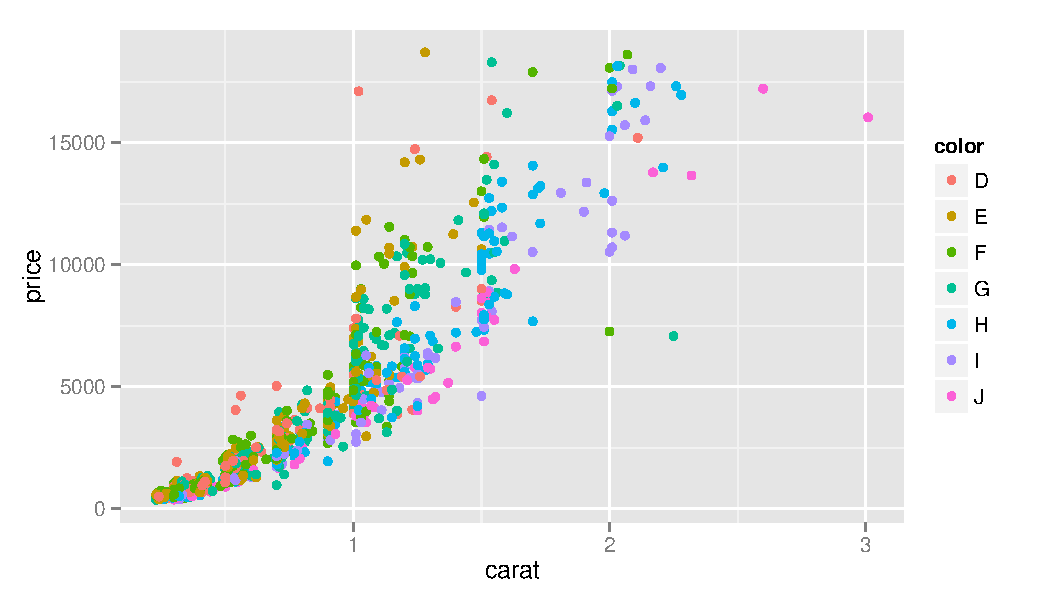
\includegraphics[width=.75\linewidth]{figure/ex1-1} 

}



\end{knitrout}
\end{frame}

% --------------------------------------------------------------
% --------------------------------------------------------------

\section*{Stats}
\frame{\sectionpage}

% --------------------------------------------------------------
% --------------------------------------------------------------

\begin{frame}[fragile]
\frametitle{Some terminology}
\begin{columns}[t]

\begin{column}[T]{3cm}
\begin{itemize}
    \item \textbf{\color{gray}data}
    \item \textbf{\color{gray}aesthetics}
    \item \textbf{\color{gray}geometry}
    \item \textbf{stat}s
\end{itemize}
\end{column}

\begin{column}[T]{8cm}
\begin{itemize}
    \item \textbf{Statistical transformations and data summary}
    \item All geoms have associated default stats, and vice versa
    \item e.g. binning for a histogram or fitting a linear model
\end{itemize}
\end{column}

\end{columns}
\end{frame}

% --------------------------------------------------------------

\begin{frame}[fragile]
\frametitle{Built-in stat example: Boxplots}
See \texttt{?geom\_boxplot} for list of options
\begin{knitrout}\footnotesize
\definecolor{shadecolor}{rgb}{0.969, 0.969, 0.969}\color{fgcolor}\begin{kframe}
\begin{alltt}
\hlkwd{library}\hlstd{(MASS)}
\hlkwd{ggplot}\hlstd{(birthwt,} \hlkwd{aes}\hlstd{(}\hlkwd{factor}\hlstd{(race), bwt))} \hlopt{+} \hlkwd{geom_boxplot}\hlstd{()}
\end{alltt}
\end{kframe}

{\centering 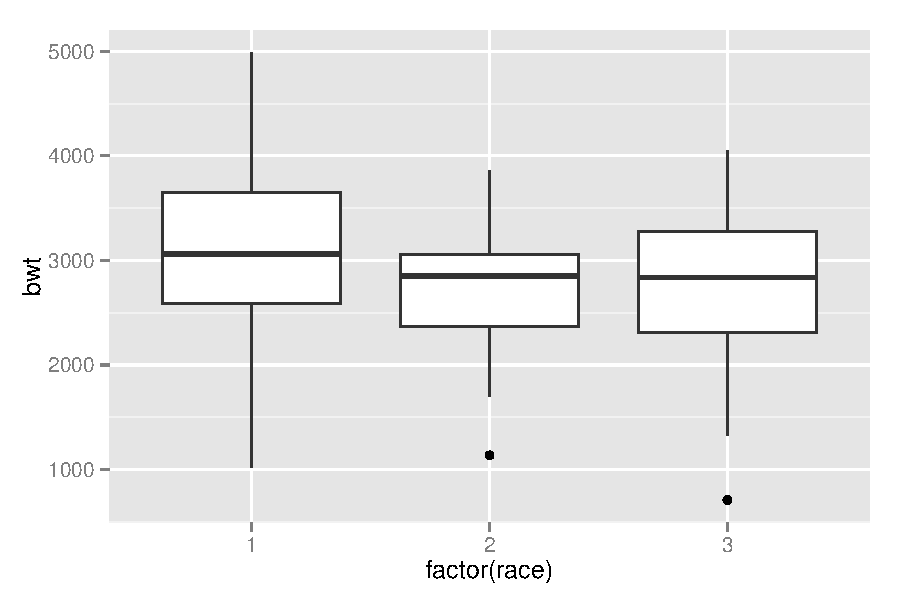
\includegraphics[width=.75\linewidth]{figure/boxplots1_-1} 

}



\end{knitrout}
\end{frame}

% --------------------------------------------------------------

\begin{frame}[fragile]
\frametitle{Built-in stat example: Boxplots}
\begin{knitrout}\footnotesize
\definecolor{shadecolor}{rgb}{0.969, 0.969, 0.969}\color{fgcolor}\begin{kframe}
\begin{alltt}
\hlstd{myplot} \hlkwb{<-} \hlkwd{ggplot}\hlstd{(birthwt,} \hlkwd{aes}\hlstd{(}\hlkwd{factor}\hlstd{(race), bwt))} \hlopt{+} \hlkwd{geom_boxplot}\hlstd{()}
\hlkwd{summary}\hlstd{(myplot)}
\end{alltt}
\begin{verbatim}
## data: low, age, lwt, race, smoke, ptl, ht, ui, ftv,
##   bwt [189x10]
## mapping:  x = factor(race), y = bwt
## faceting: facet_null() 
## -----------------------------------
## geom_boxplot: outlier.colour = black, outlier.shape = 16, outlier.size = 2, notch = FALSE, notchwidth = 0.5, varwidth = FALSE 
## stat_boxplot:  
## position_dodge: (width = NULL, height = NULL)
\end{verbatim}
\end{kframe}
\end{knitrout}
\end{frame}

% --------------------------------------------------------------
% --------------------------------------------------------------

\section*{Facets}
\frame{\sectionpage}

% --------------------------------------------------------------
% --------------------------------------------------------------


\begin{frame}[fragile]
\frametitle{Some terminology}
\begin{columns}[t]

\begin{column}[T]{3cm}
\begin{itemize}
    \item \textbf{\color{gray}data}
    \item \textbf{\color{gray}aesthetics}
    \item \textbf{\color{gray}geometry}
    \item \textbf{\color{gray}stats}
    \item \textbf{facet}s
\end{itemize}
\end{column}

\begin{column}[T]{8cm}
\begin{itemize}
    \item \textbf{Subsetting data to make lattice plots}
    \item Really powerful
\end{itemize}
\end{column}

\end{columns}
\end{frame}

% --------------------------------------------------------------

\begin{frame}[fragile]
\frametitle{Faceting: single column, multiple rows}
\begin{knitrout}\footnotesize
\definecolor{shadecolor}{rgb}{0.969, 0.969, 0.969}\color{fgcolor}\begin{kframe}
\begin{alltt}
\hlkwd{ggplot}\hlstd{(iris,} \hlkwd{aes}\hlstd{(Sepal.Length, Sepal.Width,} \hlkwc{color} \hlstd{= Species))} \hlopt{+}
    \hlkwd{geom_point}\hlstd{()} \hlopt{+}
    \hlkwd{facet_grid}\hlstd{(Species} \hlopt{~} \hlstd{.)}
\end{alltt}
\end{kframe}

{\centering 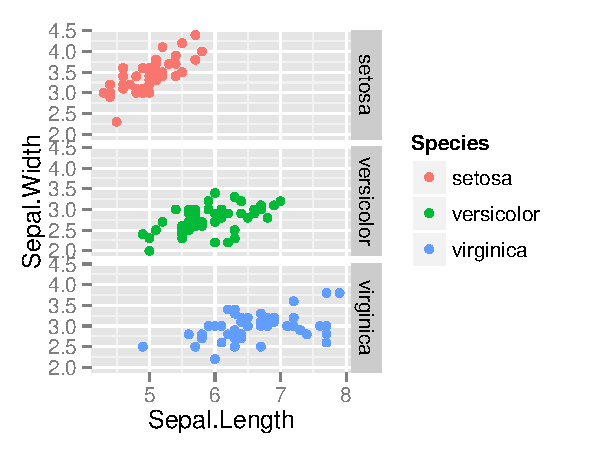
\includegraphics[width=.75\linewidth]{figure/facetgrid1-1} 

}



\end{knitrout}
\end{frame}

% --------------------------------------------------------------

\begin{frame}[fragile]
\frametitle{Faceting: single row, multiple columns}
\begin{knitrout}\footnotesize
\definecolor{shadecolor}{rgb}{0.969, 0.969, 0.969}\color{fgcolor}\begin{kframe}
\begin{alltt}
\hlkwd{ggplot}\hlstd{(iris,} \hlkwd{aes}\hlstd{(Sepal.Length, Sepal.Width,} \hlkwc{color} \hlstd{= Species))} \hlopt{+}
    \hlkwd{geom_point}\hlstd{()} \hlopt{+}
    \hlkwd{facet_grid}\hlstd{(.} \hlopt{~} \hlstd{Species)}
\end{alltt}
\end{kframe}

{\centering 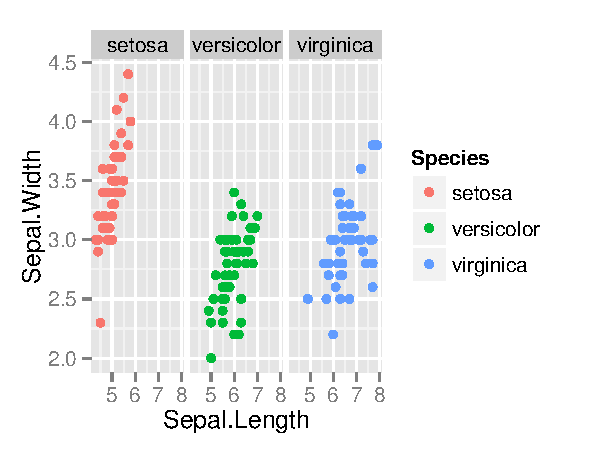
\includegraphics[width=.75\linewidth]{figure/facet_grid2-1} 

}



\end{knitrout}
\end{frame}

% --------------------------------------------------------------

\begin{frame}[fragile]
\frametitle{or just wrap your facets}
\begin{knitrout}\footnotesize
\definecolor{shadecolor}{rgb}{0.969, 0.969, 0.969}\color{fgcolor}\begin{kframe}
\begin{alltt}
\hlkwd{ggplot}\hlstd{(iris,} \hlkwd{aes}\hlstd{(Sepal.Length, Sepal.Width,} \hlkwc{color} \hlstd{= Species))} \hlopt{+}
    \hlkwd{geom_point}\hlstd{()} \hlopt{+}
    \hlkwd{facet_wrap}\hlstd{(} \hlopt{~} \hlstd{Species)} \hlcom{# notice lack of .}
\end{alltt}
\end{kframe}

{\centering 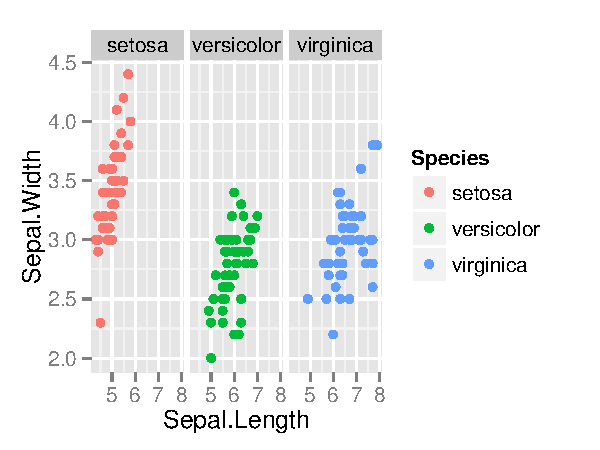
\includegraphics[width=.75\linewidth]{figure/facet_wrap-1} 

}



\end{knitrout}
\end{frame}

% --------------------------------------------------------------
% --------------------------------------------------------------

\section*{Scales}
\frame{\sectionpage}

% --------------------------------------------------------------
% --------------------------------------------------------------


\begin{frame}[fragile]
\frametitle{Some terminology}
\begin{columns}[t]

\begin{column}[T]{3cm}
\begin{itemize}
    \item \textbf{\color{gray}data}
    \item \textbf{\color{gray}aesthetics}
    \item \textbf{\color{gray}geometry}
    \item \textbf{\color{gray}stats}
    \item \textbf{\color{gray}facets}
    \item \textbf{scale}s
\end{itemize}
\end{column}

\begin{column}[T]{8cm}
\begin{itemize}
    \item \textbf{Control the mapping from data to aesthetics}
    \item Often used for adjusting color mapping
\end{itemize}
\end{column}

\end{columns}
\end{frame}

% --------------------------------------------------------------

\begin{frame}[fragile]
\frametitle{Colors}
\begin{knitrout}\footnotesize
\definecolor{shadecolor}{rgb}{0.969, 0.969, 0.969}\color{fgcolor}\begin{kframe}
\begin{alltt}
\hlkwd{aes}\hlstd{(}\hlkwc{color} \hlstd{= variable)} \hlcom{# mapping}
\hlstd{color} \hlkwb{=} \hlstr{"black"} \hlcom{# setting}

\hlcom{# Or add it as a scale}
\hlkwd{scale_fill_manual}\hlstd{(}\hlkwc{values} \hlstd{=} \hlkwd{c}\hlstd{(}\hlstr{"color1"}\hlstd{,} \hlstr{"color2"}\hlstd{))}
\end{alltt}
\end{kframe}
\end{knitrout}
\end{frame}

% --------------------------------------------------------------

\begin{frame}[fragile]
\frametitle{The RColorBrewer package}
\begin{knitrout}\footnotesize
\definecolor{shadecolor}{rgb}{0.969, 0.969, 0.969}\color{fgcolor}\begin{kframe}
\begin{alltt}
\hlkwd{library}\hlstd{(RColorBrewer)}
\hlkwd{display.brewer.all}\hlstd{()}
\end{alltt}
\end{kframe}
\end{knitrout}
\begin{center}
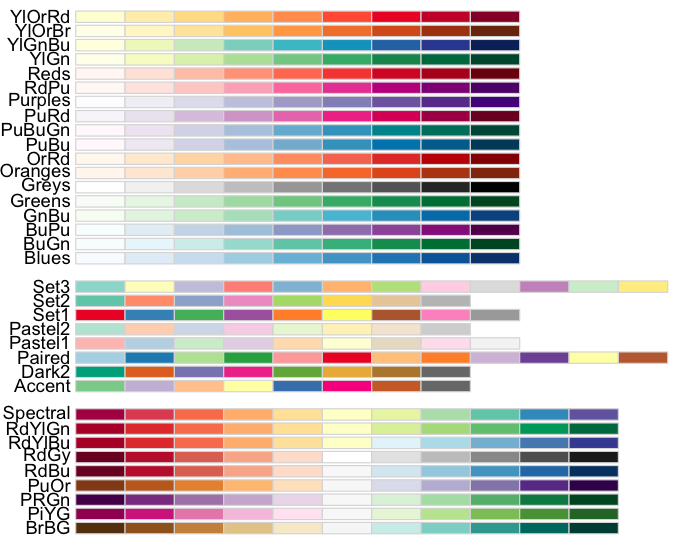
\includegraphics[scale=0.25]{images/color_palette.png}
\end{center}
\end{frame}

% --------------------------------------------------------------

\begin{frame}[fragile]
\frametitle{Using a color brewer palette}
\begin{knitrout}\footnotesize
\definecolor{shadecolor}{rgb}{0.969, 0.969, 0.969}\color{fgcolor}\begin{kframe}
\begin{alltt}
\hlstd{df}  \hlkwb{<-} \hlkwd{melt}\hlstd{(iris,} \hlkwc{id.vars} \hlstd{=} \hlstr{"Species"}\hlstd{)}
\hlkwd{ggplot}\hlstd{(df,} \hlkwd{aes}\hlstd{(Species, value,} \hlkwc{fill} \hlstd{= variable))} \hlopt{+}
    \hlkwd{geom_bar}\hlstd{(}\hlkwc{stat} \hlstd{=} \hlstr{"identity"}\hlstd{,} \hlkwc{position} \hlstd{=} \hlstr{"dodge"}\hlstd{)} \hlopt{+}
    \hlkwd{scale_fill_brewer}\hlstd{(}\hlkwc{palette} \hlstd{=} \hlstr{"Set1"}\hlstd{)}
\end{alltt}
\end{kframe}

{\centering 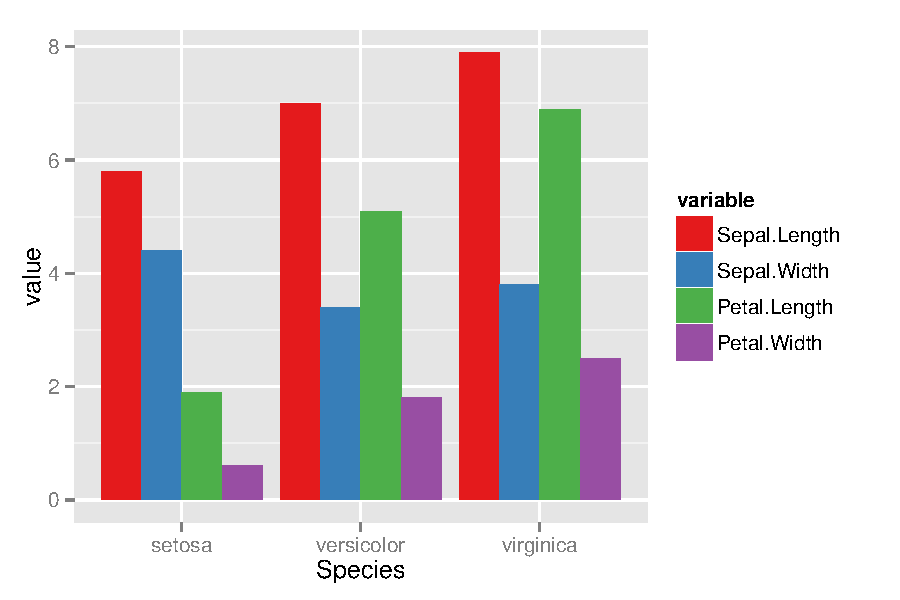
\includegraphics[width=.75\linewidth]{figure/barcolors-1} 

}



\end{knitrout}
\end{frame}

% --------------------------------------------------------------

\begin{frame}[fragile]
\frametitle{Manual color scale}
\begin{knitrout}\footnotesize
\definecolor{shadecolor}{rgb}{0.969, 0.969, 0.969}\color{fgcolor}\begin{kframe}
\begin{alltt}
\hlkwd{ggplot}\hlstd{(iris,} \hlkwd{aes}\hlstd{(Sepal.Length, Sepal.Width,} \hlkwc{color} \hlstd{= Species))} \hlopt{+}
    \hlkwd{geom_point}\hlstd{()} \hlopt{+}
    \hlkwd{facet_grid}\hlstd{(Species} \hlopt{~} \hlstd{.)} \hlopt{+}
    \hlkwd{scale_color_manual}\hlstd{(}\hlkwc{values} \hlstd{=} \hlkwd{c}\hlstd{(}\hlstr{"red"}\hlstd{,} \hlstr{"green"}\hlstd{,} \hlstr{"blue"}\hlstd{))}
\end{alltt}
\end{kframe}

{\centering 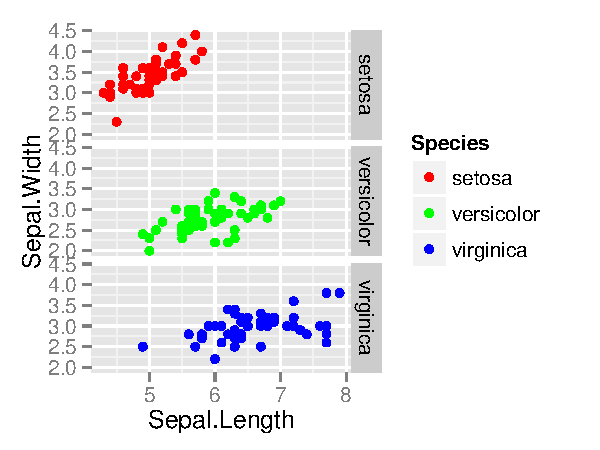
\includegraphics[width=.75\linewidth]{figure/facetgridcolors-1} 

}



\end{knitrout}
\end{frame}

% --------------------------------------------------------------

\begin{frame}[fragile]
\frametitle{Refer to a color chart for beautful visualizations}
\begin{center}
\url{http://tools.medialab.sciences-po.fr/iwanthue/}
\newline
\newline
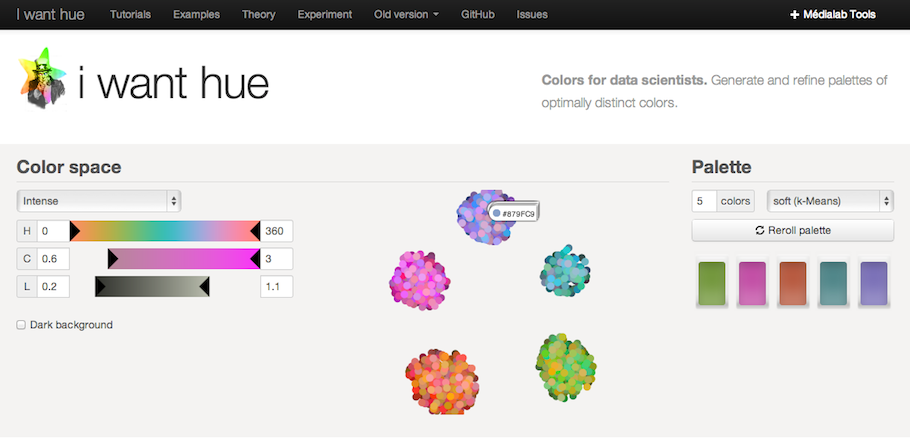
\includegraphics[scale=0.25]{images/color_schemes.png}
\end{center}
\end{frame}

% --------------------------------------------------------------

\begin{frame}[fragile]
\frametitle{Adding a continuous scale to an axis}
\begin{knitrout}\footnotesize
\definecolor{shadecolor}{rgb}{0.969, 0.969, 0.969}\color{fgcolor}\begin{kframe}
\begin{alltt}
\hlkwd{library}\hlstd{(MASS)}
\hlkwd{ggplot}\hlstd{(birthwt,} \hlkwd{aes}\hlstd{(}\hlkwd{factor}\hlstd{(race), bwt))} \hlopt{+}
    \hlkwd{geom_boxplot}\hlstd{(}\hlkwc{width} \hlstd{=} \hlnum{.2}\hlstd{)} \hlopt{+}
    \hlkwd{scale_y_continuous}\hlstd{(}\hlkwc{labels} \hlstd{= (}\hlkwd{paste0}\hlstd{(}\hlnum{1}\hlopt{:}\hlnum{4}\hlstd{,} \hlstr{" Kg"}\hlstd{)),}
        \hlkwc{breaks} \hlstd{=} \hlkwd{seq}\hlstd{(}\hlnum{1000}\hlstd{,} \hlnum{4000}\hlstd{,} \hlkwc{by} \hlstd{=} \hlnum{1000}\hlstd{))}
\end{alltt}
\end{kframe}

{\centering 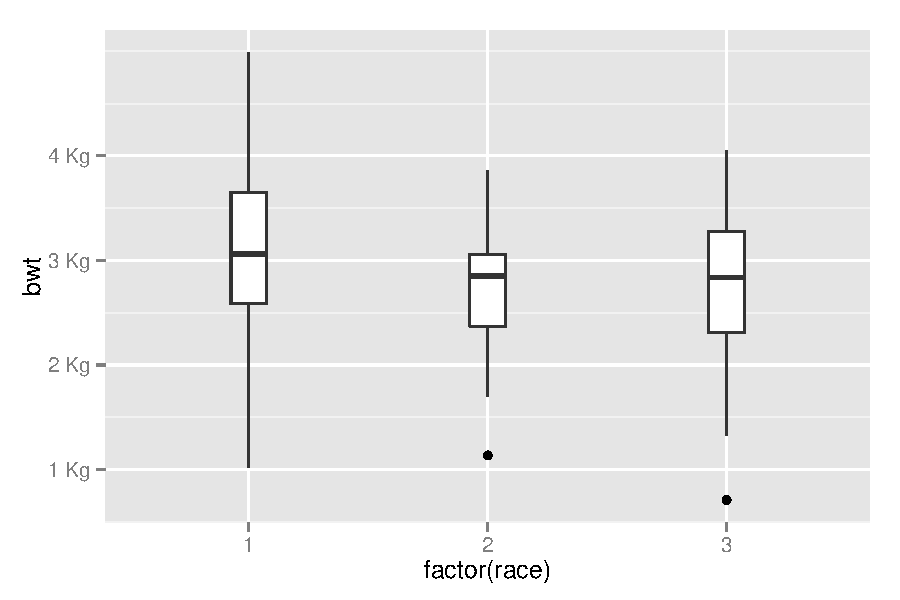
\includegraphics[width=.75\linewidth]{figure/boxplots3-1} 

}



\end{knitrout}
\end{frame}

% --------------------------------------------------------------

\begin{frame}[fragile]
\frametitle{Commonly used scales}
\begin{knitrout}\footnotesize
\definecolor{shadecolor}{rgb}{0.969, 0.969, 0.969}\color{fgcolor}\begin{kframe}
\begin{alltt}
\hlkwd{scale_fill_discrete}\hlstd{();} \hlkwd{scale_colour_discrete}\hlstd{()}
\hlkwd{scale_fill_hue}\hlstd{();} \hlkwd{scale_color_hue}\hlstd{()}
\hlkwd{scale_fill_manual}\hlstd{();}  \hlkwd{scale_color_manual}\hlstd{()}
\hlkwd{scale_fill_brewer}\hlstd{();} \hlkwd{scale_color_brewer}\hlstd{()}
\hlkwd{scale_linetype}\hlstd{();} \hlkwd{scale_shape_manual}\hlstd{()}
\end{alltt}
\end{kframe}
\end{knitrout}
\end{frame}

% --------------------------------------------------------------
% --------------------------------------------------------------

\section*{Coordinates}
\frame{\sectionpage}

% --------------------------------------------------------------
% --------------------------------------------------------------

\begin{frame}[fragile]
\frametitle{Some terminology}
\begin{columns}[t]

\begin{column}[T]{3cm}
\begin{itemize}
    \item \textbf{\color{gray}data}
    \item \textbf{\color{gray}aesthetics}
    \item \textbf{\color{gray}geometry}
    \item \textbf{\color{gray}stats}
    \item \textbf{\color{gray}facets}
    \item \textbf{\color{gray}scales}
    \item \textbf{coord}inates
\end{itemize}
\end{column}

\begin{column}[T]{8cm}
\begin{itemize}
    \item Not going to cover this in detail
    \item e.g. polar coordinate plots
\end{itemize}
\end{column}

\end{columns}
\end{frame}

% --------------------------------------------------------------
% --------------------------------------------------------------

\section*{Putting it all together with more examples}
\frame{\sectionpage}

% --------------------------------------------------------------
% --------------------------------------------------------------

\section*{Histograms}
\frame{\sectionpage}

% --------------------------------------------------------------
% --------------------------------------------------------------

\begin{frame}[fragile]
See \texttt{?geom\_histogram} for list of options
\begin{knitrout}\footnotesize
\definecolor{shadecolor}{rgb}{0.969, 0.969, 0.969}\color{fgcolor}\begin{kframe}
\begin{alltt}
\hlstd{h} \hlkwb{<-} \hlkwd{ggplot}\hlstd{(faithful,} \hlkwd{aes}\hlstd{(}\hlkwc{x} \hlstd{= waiting))}
\hlstd{h} \hlopt{+} \hlkwd{geom_histogram}\hlstd{(}\hlkwc{binwidth} \hlstd{=} \hlnum{30}\hlstd{,} \hlkwc{colour} \hlstd{=} \hlstr{"black"}\hlstd{)}
\end{alltt}
\end{kframe}

{\centering 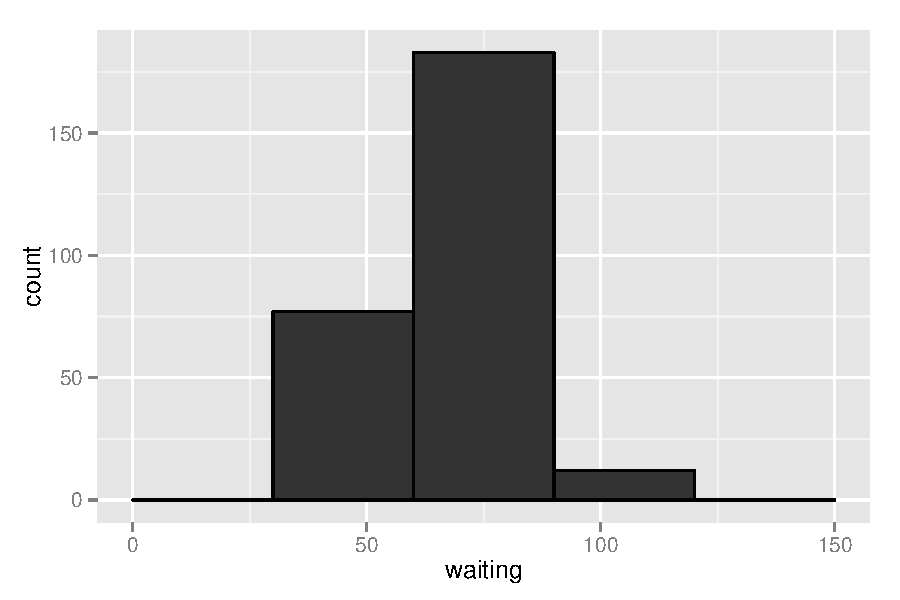
\includegraphics[width=.75\linewidth]{figure/histogr-1} 

}



\end{knitrout}
\end{frame}

% --------------------------------------------------------------

\begin{frame}[fragile]
\begin{knitrout}\footnotesize
\definecolor{shadecolor}{rgb}{0.969, 0.969, 0.969}\color{fgcolor}\begin{kframe}
\begin{alltt}
\hlstd{h} \hlkwb{<-} \hlkwd{ggplot}\hlstd{(faithful,} \hlkwd{aes}\hlstd{(}\hlkwc{x} \hlstd{= waiting))}
\hlstd{h} \hlopt{+} \hlkwd{geom_histogram}\hlstd{(}\hlkwc{binwidth} \hlstd{=} \hlnum{8}\hlstd{,} \hlkwc{fill} \hlstd{=} \hlstr{"steelblue"}\hlstd{,}
\hlkwc{colour} \hlstd{=} \hlstr{"black"}\hlstd{)}
\end{alltt}
\end{kframe}

{\centering 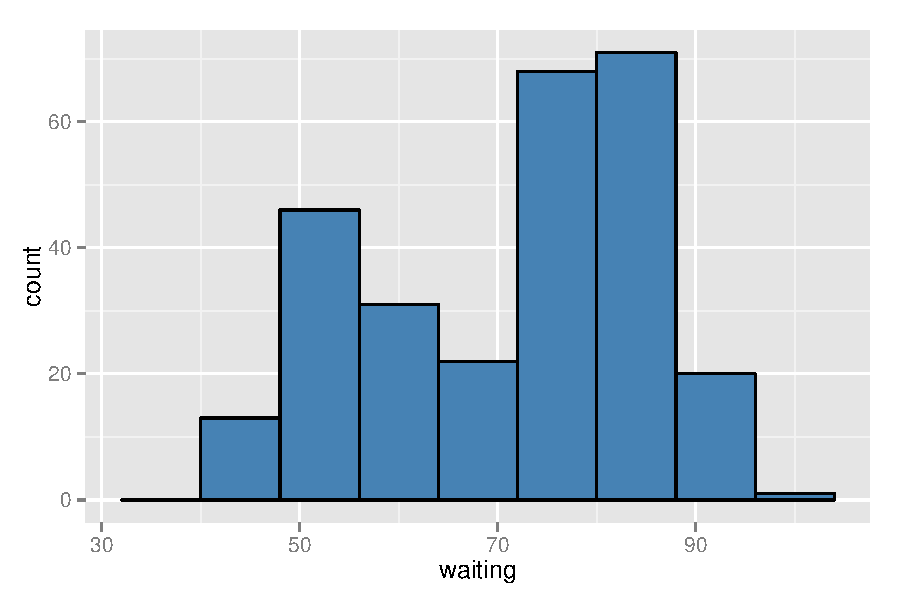
\includegraphics[width=.75\linewidth]{figure/histogra-1} 

}



\end{knitrout}
\end{frame}

% --------------------------------------------------------------
% --------------------------------------------------------------

\section*{Line plots}
\frame{\sectionpage}

% --------------------------------------------------------------
% --------------------------------------------------------------

\begin{frame}[fragile]
\begin{knitrout}\footnotesize
\definecolor{shadecolor}{rgb}{0.969, 0.969, 0.969}\color{fgcolor}\begin{kframe}
\begin{alltt}
\hlstd{climate} \hlkwb{<-} \hlkwd{read.csv}\hlstd{(}\hlstr{"../data/climate.csv"}\hlstd{,} \hlkwc{header} \hlstd{= T)}
\end{alltt}


{\ttfamily\noindent\color{warningcolor}{\#\# Warning in file(file, "{}rt"{}): cannot open file '../data/climate.csv': No such file or directory}}

{\ttfamily\noindent\bfseries\color{errorcolor}{\#\# Error in file(file, "{}rt"{}): cannot open the connection}}\begin{alltt}
\hlkwd{ggplot}\hlstd{(climate,} \hlkwd{aes}\hlstd{(Year, Anomaly10y))} \hlopt{+}
    \hlkwd{geom_line}\hlstd{()}
\end{alltt}


{\ttfamily\noindent\bfseries\color{errorcolor}{\#\# Error in ggplot(climate, aes(Year, Anomaly10y)): object 'climate' not found}}\end{kframe}
\end{knitrout}
\begin{flushright}
\begingroup
    \fontsize{6pt}{12pt}\selectfont
    \begin{verbatim}
        climate <- read.csv(text =
        RCurl::getURL('https://raw.github.com/karthikram/ggplot-lecture/master/climate.csv'))
    \end{verbatim}
\endgroup
\end{flushright}
\end{frame}

% --------------------------------------------------------------

\begin{frame}[fragile]
We can also plot confidence regions
\begin{knitrout}\footnotesize
\definecolor{shadecolor}{rgb}{0.969, 0.969, 0.969}\color{fgcolor}\begin{kframe}
\begin{alltt}
\hlkwd{ggplot}\hlstd{(climate,} \hlkwd{aes}\hlstd{(Year, Anomaly10y))} \hlopt{+}
    \hlkwd{geom_ribbon}\hlstd{(}\hlkwd{aes}\hlstd{(}\hlkwc{ymin} \hlstd{= Anomaly10y} \hlopt{-} \hlstd{Unc10y,}
        \hlkwc{ymax} \hlstd{= Anomaly10y} \hlopt{+} \hlstd{Unc10y),}
        \hlkwc{fill} \hlstd{=} \hlstr{"blue"}\hlstd{,} \hlkwc{alpha} \hlstd{=} \hlnum{.1}\hlstd{)} \hlopt{+}
    \hlkwd{geom_line}\hlstd{(}\hlkwc{color} \hlstd{=} \hlstr{"steelblue"}\hlstd{)}
\end{alltt}


{\ttfamily\noindent\bfseries\color{errorcolor}{\#\# Error in ggplot(climate, aes(Year, Anomaly10y)): object 'climate' not found}}\end{kframe}
\end{knitrout}
\end{frame}

% --------------------------------------------------------------

\begin{frame}[fragile]
\frametitle{Exercise 2}
\begin{itemize}
\item Modify the previous plot and change it such that there are three lines instead of one with a confidence band.
\begin{knitrout}\footnotesize
\definecolor{shadecolor}{rgb}{0.969, 0.969, 0.969}\color{fgcolor}\begin{kframe}


{\ttfamily\noindent\bfseries\color{errorcolor}{\#\# Error in ggplot(climate, aes(Year, Anomaly10y)): object 'climate' not found}}

{\ttfamily\noindent\bfseries\color{errorcolor}{\#\# Error in eval(expr, envir, enclos): object 'cplot' not found}}

{\ttfamily\noindent\bfseries\color{errorcolor}{\#\# Error in eval(expr, envir, enclos): object 'cplot' not found}}

{\ttfamily\noindent\bfseries\color{errorcolor}{\#\# Error in eval(expr, envir, enclos): object 'cplot' not found}}

{\ttfamily\noindent\bfseries\color{errorcolor}{\#\# Error in eval(expr, envir, enclos): object 'cplot' not found}}\end{kframe}
\end{knitrout}

\end{itemize}
\end{frame}

% --------------------------------------------------------------
% --------------------------------------------------------------

\section*{Bar plots}
\frame{\sectionpage}

% --------------------------------------------------------------
% --------------------------------------------------------------

\begin{frame}[fragile]
\begin{knitrout}\footnotesize
\definecolor{shadecolor}{rgb}{0.969, 0.969, 0.969}\color{fgcolor}\begin{kframe}
\begin{alltt}
\hlkwd{ggplot}\hlstd{(iris,} \hlkwd{aes}\hlstd{(Species, Sepal.Length))} \hlopt{+}
\hlkwd{geom_bar}\hlstd{(}\hlkwc{stat} \hlstd{=} \hlstr{"identity"}\hlstd{)}
\end{alltt}
\end{kframe}

{\centering 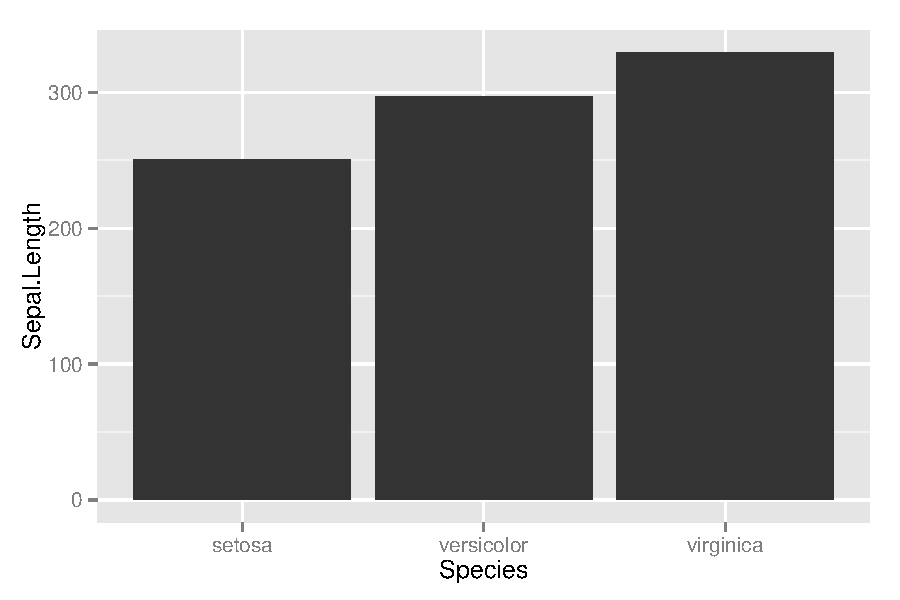
\includegraphics[width=.75\linewidth]{figure/barone-1} 

}



\end{knitrout}
\end{frame}

% --------------------------------------------------------------

\begin{frame}[fragile]
\begin{knitrout}\footnotesize
\definecolor{shadecolor}{rgb}{0.969, 0.969, 0.969}\color{fgcolor}\begin{kframe}
\begin{alltt}
\hlstd{df}  \hlkwb{<-} \hlkwd{melt}\hlstd{(iris,} \hlkwc{id.vars} \hlstd{=} \hlstr{"Species"}\hlstd{)}
\hlkwd{ggplot}\hlstd{(df,} \hlkwd{aes}\hlstd{(Species, value,} \hlkwc{fill} \hlstd{= variable))} \hlopt{+}
    \hlkwd{geom_bar}\hlstd{(}\hlkwc{stat} \hlstd{=} \hlstr{"identity"}\hlstd{)}
\end{alltt}
\end{kframe}

{\centering 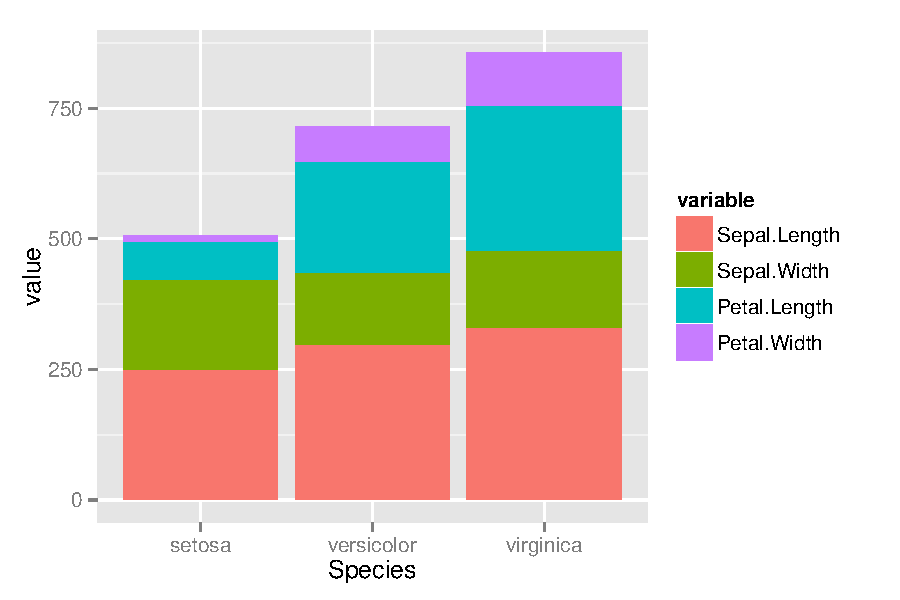
\includegraphics[width=.75\linewidth]{figure/bartwo-1} 

}



\end{knitrout}
\end{frame}

% --------------------------------------------------------------
% http://stackoverflow.com/questions/11604070/issue-with-ggplot2-geom-bar-and-position-dodge-stacked-has-correct-y-values

\begin{frame}[fragile]
\begin{knitrout}\footnotesize
\definecolor{shadecolor}{rgb}{0.969, 0.969, 0.969}\color{fgcolor}\begin{kframe}
\begin{alltt}
\hlkwd{ggplot}\hlstd{(df,} \hlkwd{aes}\hlstd{(Species, value,} \hlkwc{fill} \hlstd{= variable))} \hlopt{+}
    \hlkwd{geom_bar}\hlstd{(}\hlkwc{stat} \hlstd{=} \hlstr{"identity"}\hlstd{,} \hlkwc{position} \hlstd{=} \hlstr{"dodge"}\hlstd{)}
\end{alltt}
\end{kframe}

{\centering 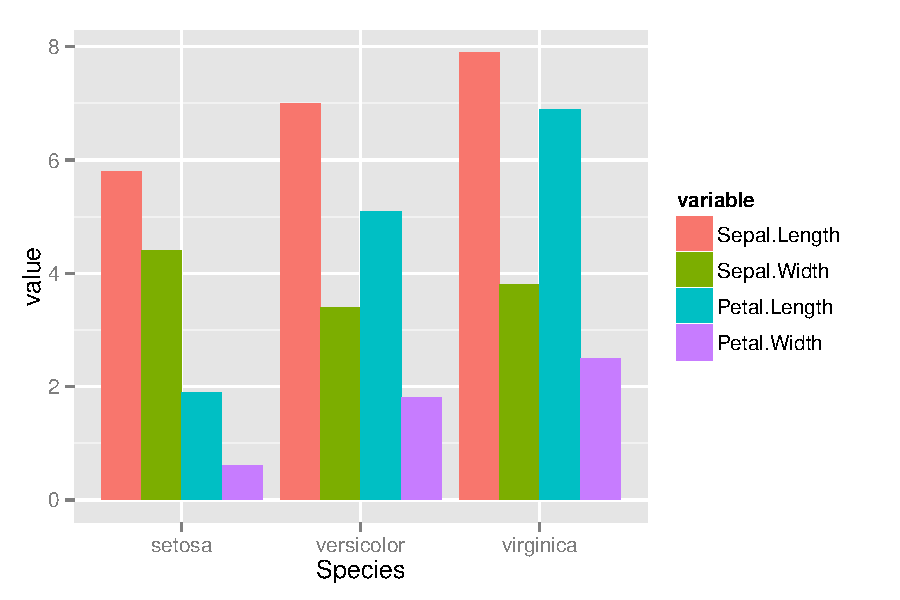
\includegraphics[width=.75\linewidth]{figure/barthree-1} 

}



\end{knitrout}
What's going on with the y axis?
\end{frame}

% --------------------------------------------------------------

\begin{frame}[fragile]
\begin{knitrout}\footnotesize
\definecolor{shadecolor}{rgb}{0.969, 0.969, 0.969}\color{fgcolor}\begin{kframe}
\begin{alltt}
\hlkwd{ggplot}\hlstd{(df,} \hlkwd{aes}\hlstd{(Species, value,} \hlkwc{fill} \hlstd{= variable))} \hlopt{+}
    \hlkwd{geom_bar}\hlstd{(}\hlkwc{stat} \hlstd{=} \hlstr{"identity"}\hlstd{,} \hlkwc{position}\hlstd{=}\hlstr{"dodge"}\hlstd{,} \hlkwc{color}\hlstd{=}\hlstr{"black"}\hlstd{)}
\end{alltt}
\end{kframe}

{\centering 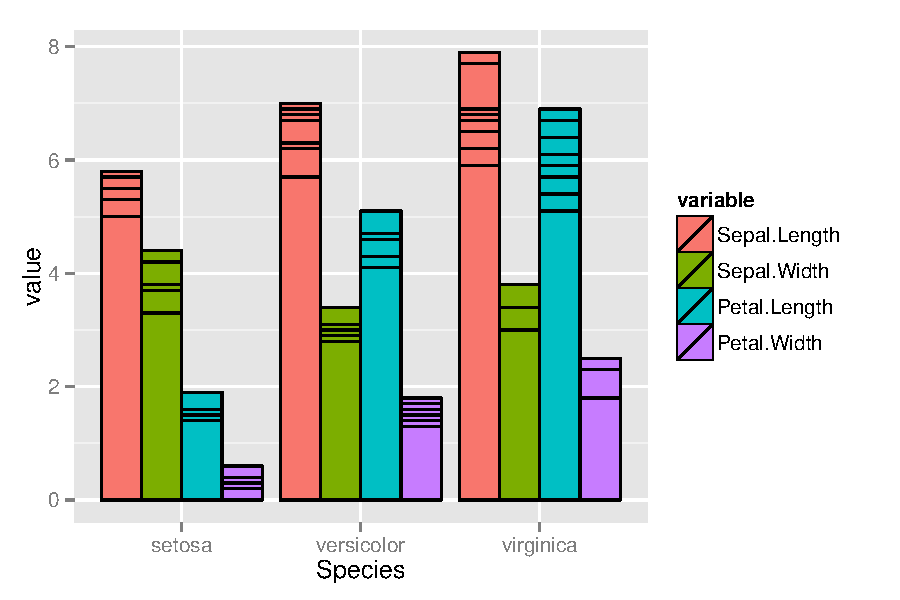
\includegraphics[width=.75\linewidth]{figure/barthree2-1} 

}



\end{knitrout}
\end{frame}

% --------------------------------------------------------------

\begin{frame}[fragile]
\frametitle{Exercise 3}
Using the d2 dataset you created earlier, generate this plot below. Take a quick look at the data first to see if it needs to be binned.
\begin{knitrout}\footnotesize
\definecolor{shadecolor}{rgb}{0.969, 0.969, 0.969}\color{fgcolor}

{\centering 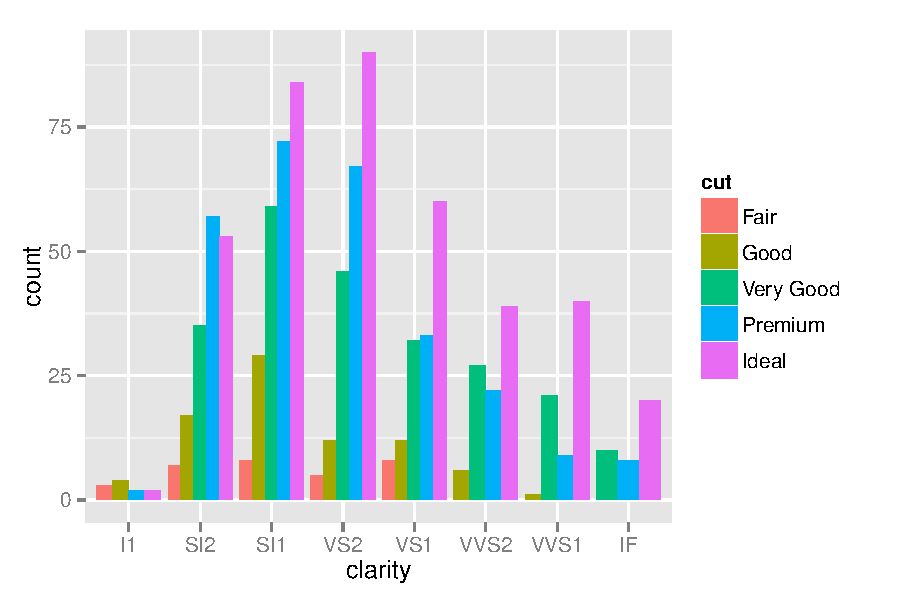
\includegraphics[width=.75\linewidth]{figure/ex3-1} 

}



\end{knitrout}
\end{frame}

% --------------------------------------------------------------

\begin{frame}[fragile]
\frametitle{Exercise 4}
\begin{itemize}
\item Using the climate dataset, create a new variable called sign. Make it logical (true/false) based on the sign of Anomaly10y.
\item Plot a bar plot and use \texttt{sign} variable as the fill.\\
\begin{knitrout}\footnotesize
\definecolor{shadecolor}{rgb}{0.969, 0.969, 0.969}\color{fgcolor}\begin{kframe}


{\ttfamily\noindent\bfseries\color{errorcolor}{\#\# Error in file(file, "{}rt"{}): cannot open the connection}}

{\ttfamily\noindent\bfseries\color{errorcolor}{\#\# Error in ifelse(clim\$Anomaly10y < 0, FALSE, TRUE): object 'clim' not found}}

{\ttfamily\noindent\bfseries\color{errorcolor}{\#\# Error in ggplot(clim, aes(Year, Anomaly10y)): object 'clim' not found}}\end{kframe}
\end{knitrout}

\end{itemize}
\end{frame}

% --------------------------------------------------------------
% --------------------------------------------------------------

\section*{Density Plots}
\frame{\sectionpage}

% --------------------------------------------------------------
% --------------------------------------------------------------

\begin{frame}[fragile]
\frametitle{Density plots}
\begin{knitrout}\footnotesize
\definecolor{shadecolor}{rgb}{0.969, 0.969, 0.969}\color{fgcolor}\begin{kframe}
\begin{alltt}
\hlkwd{ggplot}\hlstd{(faithful,} \hlkwd{aes}\hlstd{(waiting))} \hlopt{+} \hlkwd{geom_density}\hlstd{()}
\end{alltt}
\end{kframe}

{\centering 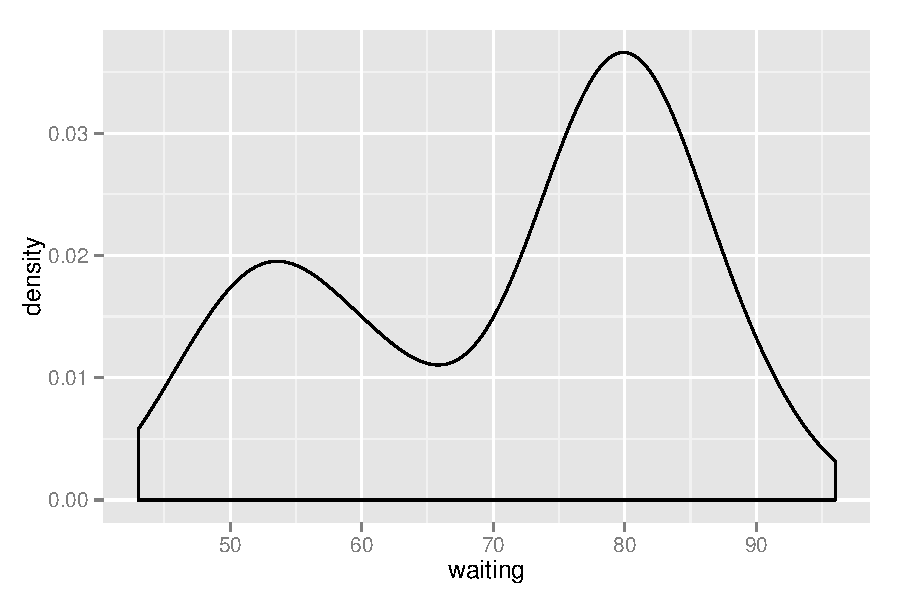
\includegraphics[width=.75\linewidth]{figure/densityone_-1} 

}



\end{knitrout}
\end{frame}

% --------------------------------------------------------------

\begin{frame}[fragile]
\frametitle{Density plots}
\begin{knitrout}\footnotesize
\definecolor{shadecolor}{rgb}{0.969, 0.969, 0.969}\color{fgcolor}\begin{kframe}
\begin{alltt}
\hlkwd{ggplot}\hlstd{(faithful,} \hlkwd{aes}\hlstd{(waiting))} \hlopt{+}
    \hlkwd{geom_density}\hlstd{(}\hlkwc{fill} \hlstd{=} \hlstr{"blue"}\hlstd{,} \hlkwc{alpha} \hlstd{=} \hlnum{0.1}\hlstd{)}
\end{alltt}
\end{kframe}

{\centering 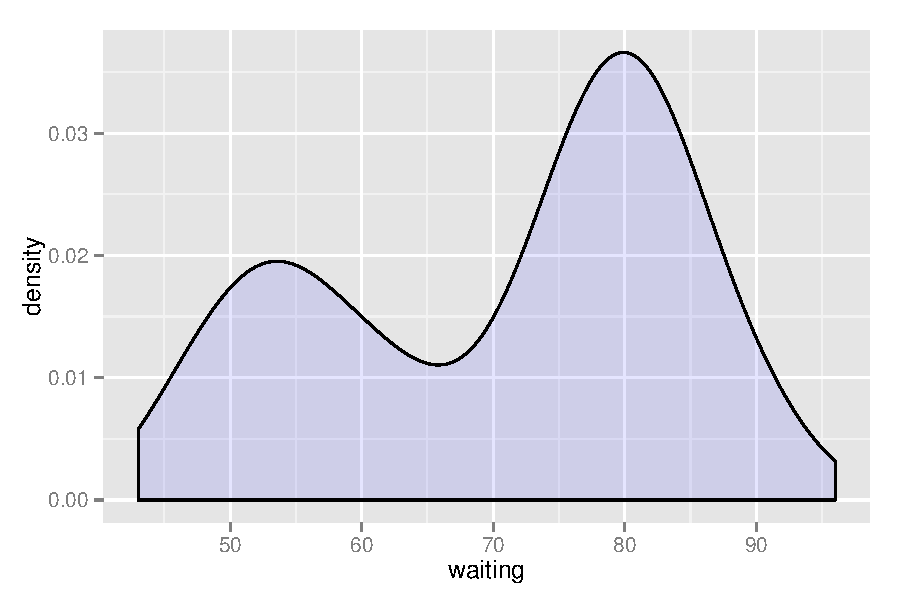
\includegraphics[width=.75\linewidth]{figure/densityonefove_-1} 

}



\end{knitrout}
\end{frame}

% --------------------------------------------------------------

\begin{frame}[fragile]
\begin{knitrout}\footnotesize
\definecolor{shadecolor}{rgb}{0.969, 0.969, 0.969}\color{fgcolor}\begin{kframe}
\begin{alltt}
\hlkwd{ggplot}\hlstd{(faithful,} \hlkwd{aes}\hlstd{(waiting))} \hlopt{+}
    \hlkwd{geom_line}\hlstd{(}\hlkwc{stat} \hlstd{=} \hlstr{"density"}\hlstd{)}
\end{alltt}
\end{kframe}

{\centering 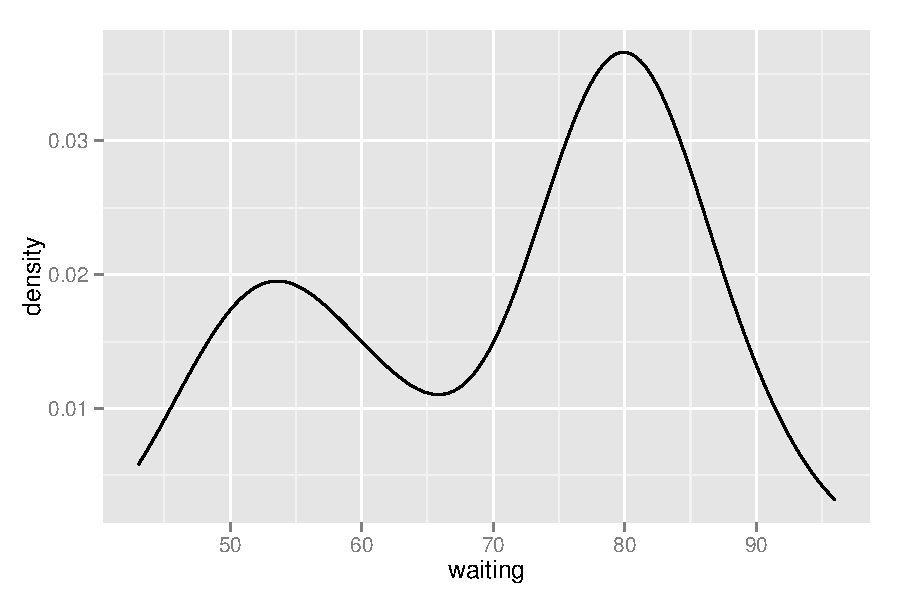
\includegraphics[width=.75\linewidth]{figure/densitytwo___-1} 

}



\end{knitrout}
\end{frame}

% --------------------------------------------------------------
% --------------------------------------------------------------

\section*{Adding smoothers}
\frame{\sectionpage}

% --------------------------------------------------------------
% --------------------------------------------------------------

\begin{frame}[fragile]
\begin{knitrout}\footnotesize
\definecolor{shadecolor}{rgb}{0.969, 0.969, 0.969}\color{fgcolor}\begin{kframe}
\begin{alltt}
\hlkwd{ggplot}\hlstd{(iris,} \hlkwd{aes}\hlstd{(Sepal.Length, Sepal.Width,} \hlkwc{color} \hlstd{= Species))} \hlopt{+}
    \hlkwd{geom_point}\hlstd{(}\hlkwd{aes}\hlstd{(}\hlkwc{shape} \hlstd{= Species),} \hlkwc{size} \hlstd{=} \hlnum{3}\hlstd{)} \hlopt{+}
    \hlkwd{geom_smooth}\hlstd{(}\hlkwc{method} \hlstd{=} \hlstr{"lm"}\hlstd{)}
\end{alltt}
\end{kframe}

{\centering 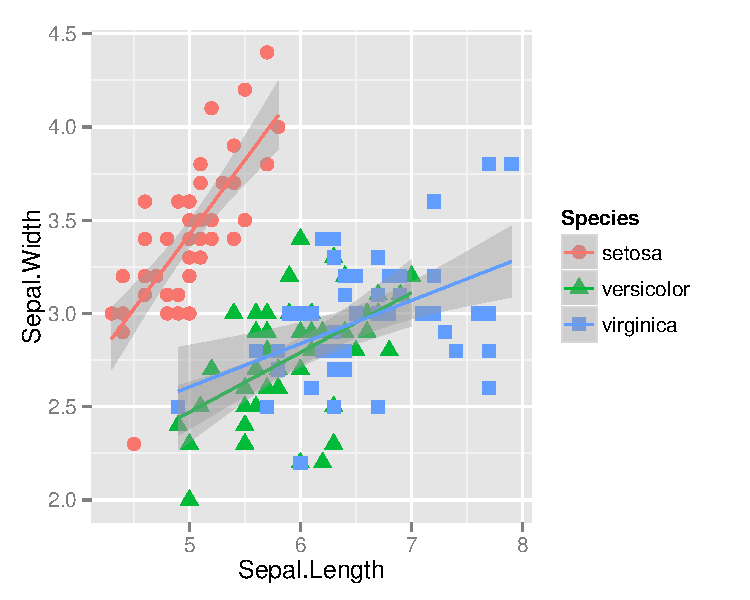
\includegraphics[width=.75\linewidth]{figure/adding_stats_-1} 

}



\end{knitrout}
\end{frame}

% --------------------------------------------------------------

\begin{frame}[fragile]
\begin{knitrout}\footnotesize
\definecolor{shadecolor}{rgb}{0.969, 0.969, 0.969}\color{fgcolor}\begin{kframe}
\begin{alltt}
\hlkwd{ggplot}\hlstd{(iris,} \hlkwd{aes}\hlstd{(Sepal.Length, Sepal.Width,} \hlkwc{color} \hlstd{= Species))} \hlopt{+}
    \hlkwd{geom_point}\hlstd{(}\hlkwd{aes}\hlstd{(}\hlkwc{shape} \hlstd{= Species),} \hlkwc{size} \hlstd{=} \hlnum{3}\hlstd{)} \hlopt{+}
    \hlkwd{geom_smooth}\hlstd{(}\hlkwc{method} \hlstd{=} \hlstr{"lm"}\hlstd{)} \hlopt{+}
    \hlkwd{facet_grid}\hlstd{(.} \hlopt{~} \hlstd{Species)}
\end{alltt}
\end{kframe}

{\centering 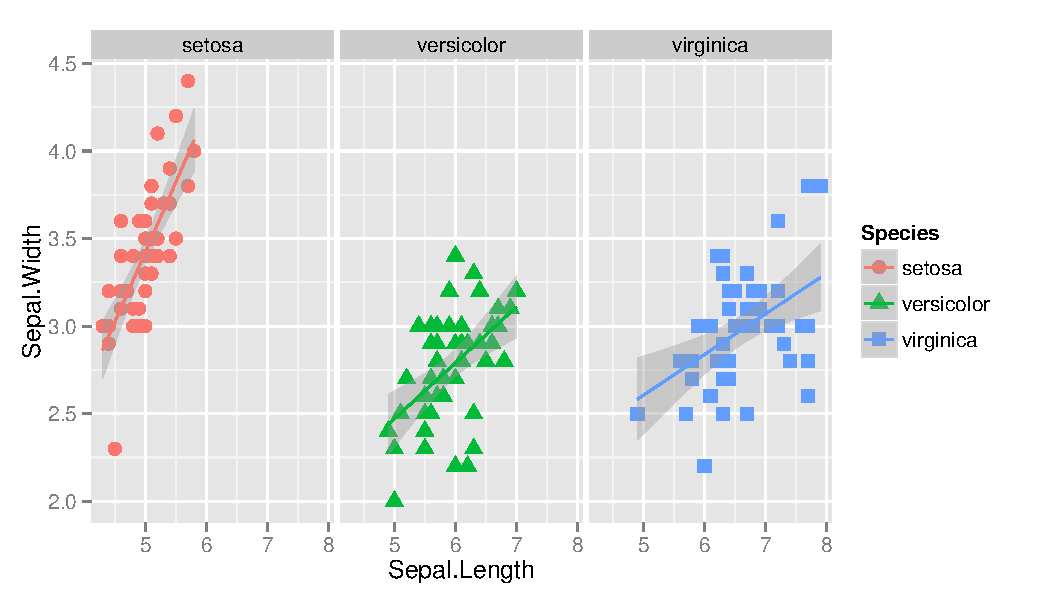
\includegraphics[width=.75\linewidth]{figure/adding_stats2_-1} 

}



\end{knitrout}
\end{frame}

% --------------------------------------------------------------
% --------------------------------------------------------------

\section*{Themes}
\frame{\sectionpage}

% --------------------------------------------------------------
% --------------------------------------------------------------

\begin{frame}[fragile]
\frametitle{Adding themes}
Themes are a great way to define custom plots.
\begin{knitrout}\footnotesize
\definecolor{shadecolor}{rgb}{0.969, 0.969, 0.969}\color{fgcolor}\begin{kframe}
\begin{alltt}
\hlopt{+} \hlkwd{theme}\hlstd{()}
\hlcom{# see ?theme() for more options}
\end{alltt}
\end{kframe}
\end{knitrout}
\end{frame}

% --------------------------------------------------------------

\begin{frame}[fragile]
\frametitle{A more basic theme}
\begin{knitrout}\footnotesize
\definecolor{shadecolor}{rgb}{0.969, 0.969, 0.969}\color{fgcolor}\begin{kframe}
\begin{alltt}
\hlkwd{ggplot}\hlstd{(iris,} \hlkwd{aes}\hlstd{(Sepal.Length, Sepal.Width,} \hlkwc{color} \hlstd{= Species))} \hlopt{+}
    \hlkwd{geom_point}\hlstd{(}\hlkwc{size} \hlstd{=} \hlnum{1.2}\hlstd{,} \hlkwc{shape} \hlstd{=} \hlnum{16}\hlstd{)} \hlopt{+}
    \hlkwd{facet_wrap}\hlstd{(} \hlopt{~} \hlstd{Species)} \hlopt{+}
    \hlkwd{theme_bw}\hlstd{()}
\end{alltt}
\end{kframe}

{\centering 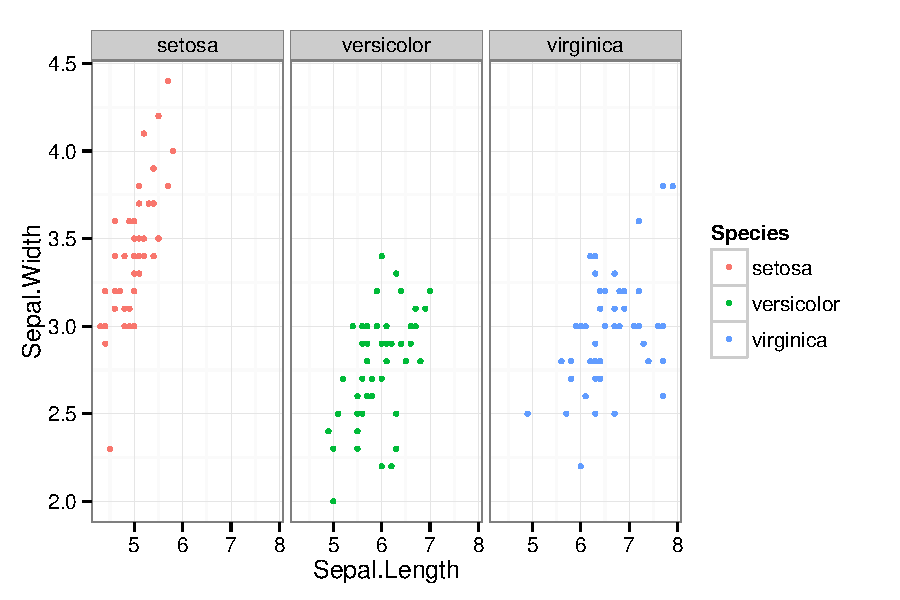
\includegraphics[width=.75\linewidth]{figure/facet_wrapbw_theme-1} 

}



\end{knitrout}
\end{frame}

% --------------------------------------------------------------

\begin{frame}[fragile]
\frametitle{A themed plot}
\begin{knitrout}\footnotesize
\definecolor{shadecolor}{rgb}{0.969, 0.969, 0.969}\color{fgcolor}\begin{kframe}
\begin{alltt}
\hlkwd{ggplot}\hlstd{(iris,} \hlkwd{aes}\hlstd{(Sepal.Length, Sepal.Width,} \hlkwc{color} \hlstd{= Species))} \hlopt{+}
    \hlkwd{geom_point}\hlstd{(}\hlkwc{size} \hlstd{=} \hlnum{1.2}\hlstd{,} \hlkwc{shape} \hlstd{=} \hlnum{16}\hlstd{)} \hlopt{+}
    \hlkwd{facet_wrap}\hlstd{(} \hlopt{~} \hlstd{Species)} \hlopt{+}
    \hlkwd{theme}\hlstd{(}\hlkwc{legend.key} \hlstd{=} \hlkwd{element_rect}\hlstd{(}\hlkwc{fill} \hlstd{=} \hlnum{NA}\hlstd{),}
        \hlkwc{legend.position} \hlstd{=} \hlstr{"bottom"}\hlstd{,}
        \hlkwc{strip.background} \hlstd{=} \hlkwd{element_rect}\hlstd{(}\hlkwc{fill} \hlstd{=} \hlnum{NA}\hlstd{),}
        \hlkwc{axis.title.y} \hlstd{=} \hlkwd{element_text}\hlstd{(}\hlkwc{angle} \hlstd{=} \hlnum{0}\hlstd{))}
\end{alltt}
\end{kframe}
\end{knitrout}
\end{frame}

% --------------------------------------------------------------

\begin{frame}[fragile]
\frametitle{A themed plot}
\begin{knitrout}\footnotesize
\definecolor{shadecolor}{rgb}{0.969, 0.969, 0.969}\color{fgcolor}
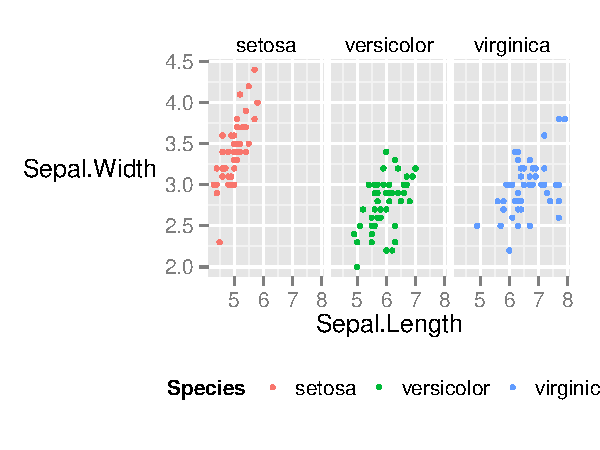
\includegraphics[width=.75\linewidth]{figure/facet_wrap_theme_execc-1} 

\end{knitrout}
\end{frame}

% --------------------------------------------------------------

\begin{frame}[fragile]
\frametitle{ggthemes library}
\begin{knitrout}\footnotesize
\definecolor{shadecolor}{rgb}{0.969, 0.969, 0.969}\color{fgcolor}\begin{kframe}
\begin{alltt}
\hlkwd{install.packages}\hlstd{(}\hlstr{'ggthemes'}\hlstd{)}
\hlkwd{library}\hlstd{(ggthemes)}
\hlcom{# Then add one of these themes to your plot}
 \hlopt{+} \hlkwd{theme_stata}\hlstd{()}
 \hlopt{+} \hlkwd{theme_excel}\hlstd{()}
 \hlopt{+} \hlkwd{theme_wsj}\hlstd{()}
 \hlopt{+} \hlkwd{theme_solarized}\hlstd{()}
\end{alltt}
\end{kframe}
\end{knitrout}
\end{frame}

% --------------------------------------------------------------

\begin{frame}[fragile]
\frametitle{Fan of Wes Anderson movies?}
\begin{center}

\includegraphics[scale=.12]{images/tenenbaums.png}
\end{center}
\end{frame}

% --------------------------------------------------------------

\begin{frame}[fragile]
\frametitle{Yup, that's a thing}
\begin{center}
\begin{knitrout}\footnotesize
\definecolor{shadecolor}{rgb}{0.969, 0.969, 0.969}\color{fgcolor}\begin{kframe}
\begin{alltt}
\hlcom{# install.packages('wesanderson')}
\hlkwd{library}\hlstd{(}\hlstr{"wesanderson"}\hlstd{)}
\hlcom{# display a palette}
\hlkwd{wes_palette}\hlstd{(}\hlstr{"Royal2"}\hlstd{,} \hlnum{5}\hlstd{)}
\end{alltt}
\end{kframe}

{\centering 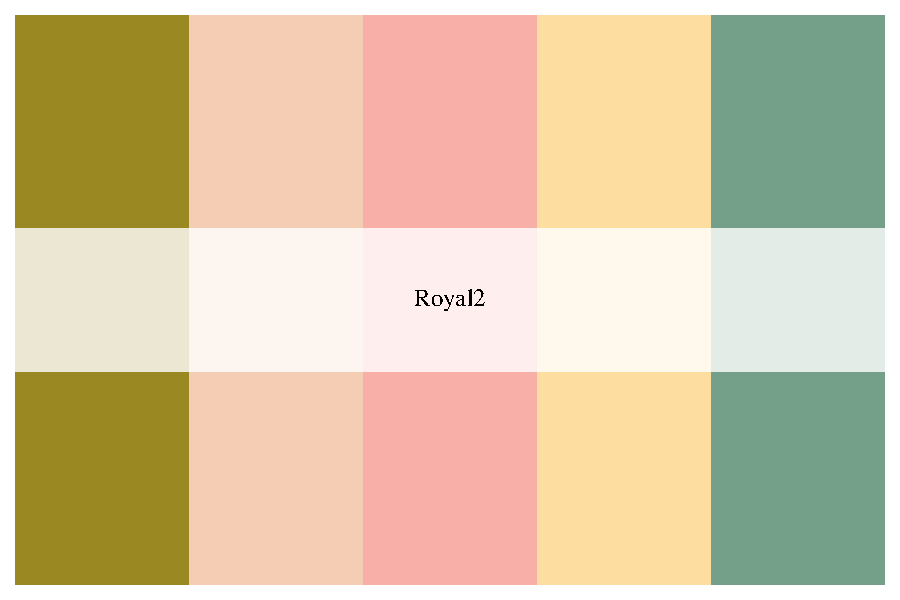
\includegraphics[width=.75\linewidth]{figure/facet_wrap_theme_exec_royal-1} 

}



\end{knitrout}
\end{center}
\end{frame}

% --------------------------------------------------------------
% --------------------------------------------------------------

\section*{Create functions to automate your plotting}
\frame{\sectionpage}

% --------------------------------------------------------------
% --------------------------------------------------------------

\begin{frame}[fragile]
\frametitle{Write functions for day to day plots}
\begin{knitrout}\footnotesize
\definecolor{shadecolor}{rgb}{0.969, 0.969, 0.969}\color{fgcolor}\begin{kframe}
\begin{alltt}
\hlstd{my_custom_plot} \hlkwb{<-} \hlkwa{function}\hlstd{(}\hlkwc{df}\hlstd{,} \hlkwc{title} \hlstd{=} \hlstr{""}\hlstd{,} \hlkwc{...}\hlstd{) \{}
    \hlkwd{ggplot}\hlstd{(df, ...)} \hlopt{+}
    \hlkwd{ggtitle}\hlstd{(title)} \hlopt{+}
    \hlkwd{whatever_geoms}\hlstd{()} \hlopt{+}
    \hlkwd{theme}\hlstd{(...)}
\hlstd{\}}
\end{alltt}
\end{kframe}
\end{knitrout}

Then just call your function to generate a plot.
It's a lot easier to fix one function that do it over and over for many plots
\begin{knitrout}\footnotesize
\definecolor{shadecolor}{rgb}{0.969, 0.969, 0.969}\color{fgcolor}\begin{kframe}
\begin{alltt}
\hlstd{plot1} \hlkwb{<-} \hlkwd{my_custom_plot}\hlstd{(dataset1,} \hlkwc{title} \hlstd{=} \hlstr{"Figure 1"}\hlstd{)}
\end{alltt}
\end{kframe}
\end{knitrout}

\end{frame}

% --------------------------------------------------------------
% --------------------------------------------------------------


\section*{Publication quality figures}
\frame{\sectionpage}

% --------------------------------------------------------------
% --------------------------------------------------------------

% How to save your plots

\begin{frame}[fragile]
\begin{itemize}
\item If the plot is on your screen
\begin{knitrout}\footnotesize
\definecolor{shadecolor}{rgb}{0.969, 0.969, 0.969}\color{fgcolor}\begin{kframe}
\begin{alltt}
\hlkwd{ggsave}\hlstd{(}\hlstr{'~/path/to/figure/filename.png'}\hlstd{)}
\end{alltt}
\end{kframe}
\end{knitrout}
\item If your plot is assigned to an object
\begin{knitrout}\footnotesize
\definecolor{shadecolor}{rgb}{0.969, 0.969, 0.969}\color{fgcolor}\begin{kframe}
\begin{alltt}
\hlkwd{ggsave}\hlstd{(plot1,} \hlkwc{file} \hlstd{=} \hlstr{"~/path/to/figure/filename.png"}\hlstd{)}
\end{alltt}
\end{kframe}
\end{knitrout}

\item Specify a size
\begin{knitrout}\footnotesize
\definecolor{shadecolor}{rgb}{0.969, 0.969, 0.969}\color{fgcolor}\begin{kframe}
\begin{alltt}
\hlkwd{ggsave}\hlstd{(}\hlkwc{file} \hlstd{=} \hlstr{"/path/to/figure/filename.png"}\hlstd{,} \hlkwc{width} \hlstd{=} \hlnum{6}\hlstd{,}
\hlkwc{height} \hlstd{=}\hlnum{4}\hlstd{)}
\end{alltt}
\end{kframe}
\end{knitrout}
\item or any format (pdf, png, eps, svg, jpg)
\begin{knitrout}\footnotesize
\definecolor{shadecolor}{rgb}{0.969, 0.969, 0.969}\color{fgcolor}\begin{kframe}
\begin{alltt}
\hlkwd{ggsave}\hlstd{(}\hlkwc{file} \hlstd{=} \hlstr{"/path/to/figure/filename.eps"}\hlstd{)}
\hlkwd{ggsave}\hlstd{(}\hlkwc{file} \hlstd{=} \hlstr{"/path/to/figure/filename.jpg"}\hlstd{)}
\hlkwd{ggsave}\hlstd{(}\hlkwc{file} \hlstd{=} \hlstr{"/path/to/figure/filename.pdf"}\hlstd{)}
\end{alltt}
\end{kframe}
\end{knitrout}
\end{itemize}
\end{frame}

% --------------------------------------------------------------

\begin{frame}[fragile]
\frametitle{Further help}
\begin{itemize}
\item You've just scratched the surface with ggplot2.
\item Practice
\item Read the docs (either locally in \texttt{R} or at \url{http://docs.ggplot2.org/current/})
\item Work together
\end{itemize}
\begin{center}

\includegraphics[scale=.15]{images/chang_book.png}
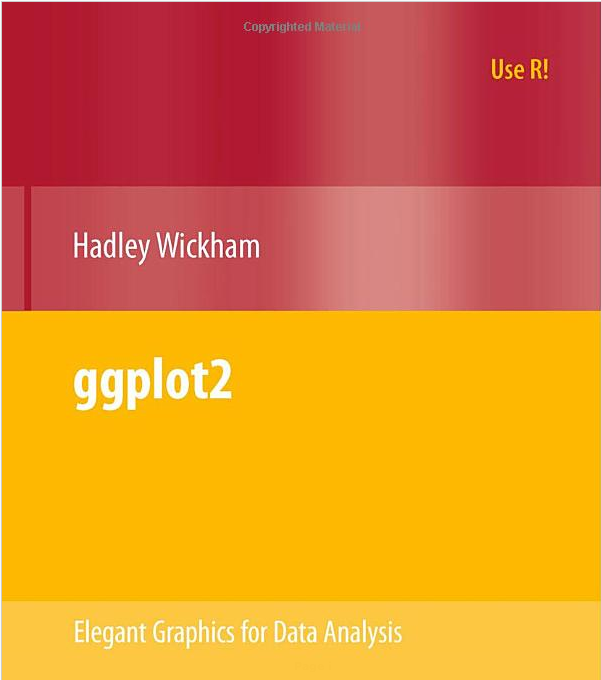
\includegraphics[scale=.15]{images/hadley.png}
\end{center}
\end{frame}

% --------------------------------------------------------------
% end, hope it was useful.
\end{document}
